\documentclass[journal]{IEEEtran}
\usepackage[T1]{fontenc}
\usepackage[utf8]{inputenc}
\usepackage[polish]{babel} % TODO:(mati): delete this line for proper autogeneration of english headers
\usepackage{graphicx}
\usepackage{subcaption}
\usepackage{hyperref}
\pagestyle{plain}
\setlength{\parskip}{0.7em}  
\setlength{\parindent}{15pt}


\ifCLASSINFOpdf
  
\else
 
\fi





% correct bad hyphenation here
\hyphenation{op-tical net-works semi-conduc-tor}


\begin{document}
\title{Analysis of heart rate variability using mobile devices and mashine learning}
\author{
    J. Bancerewicz, J. Kotłowski, O. Lozovyy, J. Morawska, M. Rzęsa\\
    \textit{Gdańsk University of Technology}\\
    \textit{Faculty of Electronics, Telecoummunications and Informatics}



% The paper headers
\markboth{}%
{Shell \MakeLowercase{\textit{et al.}}: Bare Demo of IEEEtran.cls for IEEE Journals}
\maketitle

\begin{abstract}
% TODO:(mati): i don't like translating "tłumienie zakłóceń" as noise suppression 
% TODO:(mati): proces -> approach?
This paper presents methods of analysis of heart rate variability based on electrocardiographical and photoplethysmographical signals obtained through the usage of mobile devices. An approach to processing the saved data involving noise suppression, peak detection and determining the intervals between impulses in the bodily processes has been developed. Detection of R peaks in ECG and maximums of a PPG wave has been realized using convolutional and recursive neural networks. The efficiency of the models has been measured in comparison to the classic algorithms and reference data. The results show a high accuracy of peak identification and allow employing mobile devies to monitor cardiographical parameters in both home envionments as well as during physical activities.

% W niniejszej pracy przedstawiono metody analizy zmienności rytmu serca na podstawie sygnałów elektrokardiograficznych i fotopletyzmograficznych pozyskiwanych za pomocą urządzeń przenośnych. Opracowano proces przetwarzania zapisów obejmujący tłumienie zakłóceń, wykrywanie pików oraz wyznaczanie interwałów między impulsami w przebiegu fizjologicznym. Detekcję szczytów R w EKG oraz maksimów fali w PPG zrealizowano z wykorzystaniem splotowych i rekurencyjnych sieci neuronowych. Skuteczność modeli oceniono w odniesieniu do klasycznych algorytmów jak i danych referencyjnych. Wyniki wykazały wysoką dokładność identyfikacji pików oraz umożliwiają zastosowanie mobilnych systemów do monitorowania parametrów kardiologicznych w warunkach domowych i podczas aktywności fizycznej.

% TODO:(mati): confirm the translation of these
\textbf{Keywords---} heart rate variability; biomedical signals; electrocardiography; photoplethysmography; noise filtering; convolutional neural networks; peak detection; pulse-transit time; Pan-Tompkins algorithm; time analysis.
\end{abstract}
% zmienność rytmu serca; sygnały biomedyczne; elektrokardiografia; fotopletyzmografia; filtracja sygnałów; splotowe sieci neuronowe; detekcja szczytów; interwał propagacji tętna; algorytm Pan-Tompkins; analiza czasowa.

\section{Introduction}
% TODO:(mati): ocena funkcjonowania -> assesing the health?
% TODO:(mati): czas rejestracji -> registration time? sounds dumb
Heart rate variability is an important parameter of assesing the health of the cardiovascular system as it mirrors the balance between the sympathetic and parasympathetic nervous system. Traditional HRV measurements performed in clinical conditions are characterized by their high cost and limited registration time. In recent years technological developments in the mobile devices area have made it possible to monitor the cardiographical activity in every-day life.
% Zmienność rytmu serca stanowi istotny parametr oceny funkcjonowania układu sercowo-naczyniowego, odzwierciedlający równowagę pomiędzy aktywnością układu współczulnego i przywspółczulnego. Tradycyjne pomiary HRV prowadzone w warunkach klinicznych charakteryzują się wysokim kosztem oraz ograniczonym czasem rejestracji. W ostatnich latach postęp technologiczny w obszarze urządzeń przenośnych oraz sensorów optycznych umożliwił monitorowanie aktywności kardiologicznej w trakcie życia codziennego.

% TODO:(mati): cel pracy -> goal of the paper? praca is paper in this context but is goal the best translation?
\subsection{The goal of the paper}
% TODO:(mati): zapisy -> records?
% TODO:(mati): wzorców referencyjnych -> referencial patterns?
Beat detection techniques in electrocardiographical and photoplethysmographical records are implemented and rated by their usefullness in the heart rate variability analysis. Classical algorithms are juxtaposed with soulutions based on deep neural networks including their accuracy, resistance to noise and usage in real-world conditions. An andriod mobile app registers the PPG. ECG data is acquired through a Polar H10 heart monitor. Both employ filtration, characteristic points identification as well as computing the HRV indicator. The quality of the signals obtained through the mobile devices is verified based on referential patterns. Heart rate parameters are compared with the electrocardiograph and precision of peak detection is computed.
% Techniki detekcji uderzeń w zapisach elektrokardiograficznych i fotopletyzmograficznych są implementowane i oceniane względem użyteczności w analizie zmienności rytmu serca. Klasyczne algorytmy zestawia się z rozwiązaniami opartymi na głębokich sieciach neuronowych, uwzględniając skuteczność, odporność na zakłócenia oraz zastosowanie w warunkach rzeczywistych. Aplikacja mobilna rejestruje przebiegi PPG na platformie Android, dane EKG odczytuje się z pulsometru Polar H10, wykorzystując filtrację, identyfikację punktów charakterystycznych oraz wyznaczanie wskaźników HRV. Jakość sygnałów pozyskiwanych urządzeniami mobilnymi jest weryfikowana na podstawie wzorców referencyjnych, porównując parametry rytmu serca z elektrokardiogramu i określając precyzję wykrywania szczytów.

\newpage
% Techniki filtracji i modelowania sygnałów biomedycznych
\section{Filtration and biomedical signals modeling techniques}
% TODO:(mati): process of record processing masło jest maśłane
Electrocardiography and photoplethysmography are one of the most basic sources of biomedical signals used in modern diagnostic and monitoring systems. The process of record processing is oriented towards ensuring the credibility of the bodily data in the presence of interference in the form of movement of the patient, enviornmental noise and hardware limitations. There are to dominant approaches: data filtration and artificial inteligencje modeling. These two are combined to improve the accuracy and robustness of the analysis in medical conditions \cite{1}.
% Elektrokardiografia i fotopletyzmografia należą do podstawowych źródeł sygnałów biomedycznych wykorzystywanych w nowoczesnych systemach diagnostycznych i monitorujących. Proces przetwarzania zapisów jest ukierunkowany na uzyskanie wiarygodnych informacji fizjologicznych przy obecności zakłóceń wynikających z ruchu pacjenta, interferencji środowiskowych i ograniczeń sprzętowych. Dominują dwa podejścia: filtrację danych oraz modelowanie wspierane sztuczną inteligencją, które są łączone  dla poprawy dokładności i zwiększenia odporności analizy w warunkach medycznych \cite{1}.

% Filtracja danych
\subsection{Data filtration}
% TODO:(mati): find a good synonym to processsing
% TODO:(mati): niedokładność pomiarowa -> measurement error?
% TODO:(mati): dryft linii izoelektrycznej?
Initial processing of bodily processes are based on interference elimination improving the ratio of signal to noise. Measurement error related to movement, network components with a frequency of 50/60_Hz and izoelectric drift line all play important roles in electrocardiography and photoplethysmography \cite{2}. Filtration increases the quality of the record and improves the accuracy of feature detection as well as the classification efficiency.
% Wstępne przetwarzanie przebiegów fizjologicznych opiera się na eliminacji zakłóceń, umożliwiając poprawę stosunku sygnału do szumu. W elektrokardiografii oraz fotopletyzmografii istotną rolę odgrywają niedokładności pomiarowe związane z ruchem, składowe sieciowe o częstotliwości 50/60 Hz oraz dryft linii izoelektrycznej \cite{2}. Filtracja podnosi jakość zapisu, poprawiając dokładność detekcji cech oraz efektywność klasyfikacji.

% NOTE:(mati): i translatd przebieg as measurement, it feels wrong but i can't find a better translation
% TODO:(mati): the second sentence is weird
% TODO:(mati): liniowa charakterystyka fazowa -> linear phase response?
A band-pass filter limiting the band frequency to values characteristic to the given measurement is a basic signal analysis method. Processing range comes to 0.5-40 Hz for an ECG record and 0.3-8 Hz for a PPG record correlating to the heart rate \cite{3}. Butterworth, and eliptic in the IIR and FIR form modeled using the window method and Chebyshev filters are all used in digital imlpementations providing stability and linear phase response \cite{4}.
% Do podstawowych metod analizy sygnału należą filtry pasmowoprzepustowe, ograniczające pasmo częstotliwości do wartości charakterystycznych dla badanego przebiegu. Zakres przetwarzania zapisu EKG wynosi 0,5–40 Hz, natomiast PPG ogranicza się do 0,3–8 Hz, odpowiadającego rytmowi serca \cite{3}. W implementacjach cyfrowych wykorzystuje się filtry Butterwortha, Chebysheva, eliptyczne w postaci IIR oraz FIR projektowane metodą okienkową, zapewniające stabilność i liniową charakterystykę fazową \cite{4}. 

% TODO:(mati): second sentence is a monster, i think i translated it well but it's a very complicated sentence
% NOTE:(mati): i translated eliminacja as cancellation based on the citation
Adaptive filters are used for signals containing disturbances with varying parameters. LMS and RLS algorithms allow for a dynamic adaptation of system coefficients for record characterisric which increases the effectiveness of movements instabiliteis and network interferences suppression. Notch mechanisms ensure the cancellation of the 50/60_Hz component \cite{5}.
% Dla sygnałów z zakłóceniami o zmiennych parametrach stosuje się filtry adaptacyjne. Algorytmy LMS i RLS umożliwiają dynamiczną adaptację współczynników układu do charakterystyki zapisu, zwiększając skuteczność tłumienia niestabilności ruchowych oraz interferencji sieciowych. W zastosowaniach medycznych mechanizmy notch zapewniają eliminację składowej 50/60 Hz \cite{5}.

\newpage
% TODO:(mati): eliminacja artefaktów impulsowych i krótkotrwałych?
% TODO:(mati): metody morfologiczne -> morphological methods?
% TODO:(mati): załamki QRS -> QRS waves?
Pulse and short-term impulse artifacts cancellation is realized based on a median filter as well as morphological methods which allow for preservation of diagnostic features such as QRS waves \cite{6}. Empirical Mode Decompopsition, Wavelet Packet Transform techniques and wavelet analysis provide a signal decomposition to frequency components and selective noise suppression while maintaining the measurement peaks structure \cite{7}.
% Eliminacja artefaktów impulsowych i krótkotrwałych jest realizowana w oparciu o filtry medianowe oraz metody morfologiczne, umożliwiające zachowanie cech diagnostycznych, takich jak załamki QRS \cite{6}. Analiza falkowa oraz techniki Empirical Mode Decomposition i Wavelet Packet Transform zapewniają dekompozycję sygnału na składowe częstotliwościowe oraz selektywne tłumienie szumów przy utrzymaniu struktury pików przebiegu \cite{7}.

In advanced biomedical appliances algorithms based on probabilistic models are used. One of the available methods is the Kalman filter used to estimate actual measurement based on observations influenced by noise \cite{8}. Another method is Independent Component Analysis employed to separate record sources and eliminate movement ditortions in photoplethysmography  \cite{9}. Modern dat isolation techinques combine traditional computing with mashine learning. The process of signal refining precedes extracting the features using neural networks which increases the robustness of the analysis in natural conditions \cite{10}.
% W zaawansowanych zastosowaniach biomedycznych wykorzystuje się algorytmy oparte na modelach probabilistycznych. Jedną z metod jest filtr Kalmana, służący do estymacji rzeczywistego przebiegu na podstawie obserwacji obarczonych zakłóceniami \cite{8}, oraz Independent Component Analysis, stosowaną do separacji źródeł zapisu i eliminacji zniekształceń ruchowych w fotopletyzmografii \cite{9}. Współczesne techniki wyodrębniania danych integrują tradycyjne przetwarzanie z uczeniem maszynowym. Proces oczyszczania sygnału jest etapem poprzedzającym ekstrakcję cech z użyciem sieci neuronowych, zwiększając odporność analizy w warunkach naturalnych \cite{10}.

\subsection{Uczenie maszynowe}
Artificial inteligence-based techniques are one of the key biomedical signal analysis methods. Usage of algorithms allows automatic information isolation, limits the influence of preprocessing and increases the efficiency of slissification in the presence of interference. Literature highlights three main solutions.
% Techniki oparte na sztucznej inteligencji należą do kluczowych metod analizy sygnałów biomedycznych. Zastosowanie algorytmów umożliwia automatyczne wyodrębnianie informacji, ogranicza wpływ wstępnego przetwarzania i zwiększa skuteczność klasyfikacji w obecności zniekształceń. W literaturze wyróżnia się trzy główne rozwiązania.

Supervised approaches including Support Vector Machines, k-Nearest Neighbours and Random Forest are all used to measure the heart rate and detect arythmia. Logistical regression and linear discriminant models ensures a simple and effective signal pattern identification.
Implementation of these solutions in mobile diagnostic systems and monitoring devices as well as processing in real-time is made possible by the low time complexity of aforementioned solutions \cite{11}.
%Nadzorowane podejścia, obejmujące Support Vector Machines, k-Nearest Neighbors oraz Random Forest, są wykorzystywane do oceny rytmu serca oraz detekcji arytmii. Regresja logistyczna i liniowe modele dyskryminacyjne zapewniają prostą i efektywną identyfikację wzorców sygnałów.
%Niska złożoność obliczeniowa tych rozwiązań sprzyja implementacji w przenośnych systemach diagnostycznych i urządzeniach monitorujących, wspierając przetwarzanie danych w czasie rzeczywistym \cite{11}.

A focus on sequential model is placed in the second area. They allow to replicated time dependencies in electrocardiographical and photoplethysmographical records.
Recursive neural networks and their extended forms including Long Short-Term Memory and Gated Recurrent Units register both short-term as well as long-term changes in the signal \cite{12}. Probabilistic models such as Hidden Markov Models are used alternatively to help identify anomalies and improve the efficiency of both dynamic heart rate analysis as well as cardiological abnormalities detection \cite{13}.
% Drugi obszar koncentruje się na modelach sekwencyjnych, umożliwiających odwzorowanie zależności czasowych w zapisach elektrokardiograficznych oraz fotopletyzmograficznych.
% Rekurencyjne sieci neuronowe i ich rozszerzone formy, w tym długa krótkoterminowa pamięć LSTM oraz jednostki z bramkowaniem pamięci GRU, rejestrują zarówno krótkotrwałe, jak i długookresowe zmiany sygnału \cite{12}. Alternatywnie są stosowane techniki probabilistyczne, w szczególności ukryte modele Markowa HMM, wspierające identyfikację anomalii oraz poprawiające skuteczność analizy dynamiki rytmu serca i detekcji nieprawidłowości kardiologicznych \cite{13}.

\newpage
% TODO:(mati): transformer -> transformator?
% TODO:(mati): mehcanizm uwagi -> attention mechanism?
An often used solution is the deep learning architecture which includes convolutional neural networks used to extract lokal features such as peak detection in PPG measurement and QRS complexes in ECG signal \cite{14}. Transformator based on attention mechanism provides parallel mapping of time dependencies in many scales increasing the system's robustness against movement interferences and amplitude variability \cite{15}. Hybrid solutions in which convolutional layers are combined with recursive ones integrating both local and global solutions in a single system gain increasing relevance.
% Do najczęściej wykorzystywanych rozwiązań zalicza się architektury głębokiego uczenia, w tym konwolucyjne sieci neuronowe, przeznaczone do ekstrakcji cech lokalnych, takich jak detekcja szczytów w przebiegu PPG oraz zespołów QRS w sygnale EKG \cite{14}. Transformer, oparty na mechanizmie uwagi, zapewnia równoległe odwzorowanie zależności czasowych w wielu skalach, zwiększając odporność systemów na zakłócenia ruchowe i zmienność amplitudy \cite{15}. Rosnące znaczenie zyskują rozwiązania hybrydowe, w których warstwy splotowe są łączone z rekurencyjnymi, integrujące analizę lokalną i globalną w jednym układzie.


High resistance to interferences and adaption to new data sets are both characteristic features of mashine learning. Transformation of models trained on big referencial bases to real-world clinical conditions is realized by employing the transfer solution, improving the generalization and precision of the classification \cite{16}.
%Uczenie maszynowe charakteryzuje się wysoką odpornością na zniekształcenia oraz adaptację do nowych zbiorów danych. Stosowanie podejścia transferowego realizuje przekształcenie modeli wytrenowanych na dużych bazach referencyjnych, do rzeczywistych warunków klinicznych, poprawiając generalizację oraz precyzję klasyfikacji \cite{16}.

% Ocena zmienności rytmu serca na podstawie przebiegów EKG i PPG
% TODO:(mati): second sentence is hell; is the translation accurate?
\subsection{Heart rate variability assesment based on ECG and PPG measurements}
Photoplethysmographic signals are commonly applied to estimate heart rate while electrocardiography fills the role of the referencial standard. Datasets facillitated by multichannel PPG datasets with parallel ECG record research and ultra-short-term HRV analysis using deep learning algotithms are both featured in the literature.
%Sygnały fotopletyzmograficzne są powszechnie stosowane do estymacji tętna, natomiast elektrokardiografia pełni rolę standardu referencyjnego. W literaturze wyróżnia się badania poświęcone ultra-krótkoterminowej analizie HRV z wykorzystaniem głębokiego uczenia oraz prace udostępniające obszerne, wielokanałowe zbiory danych PPG z równoległym zapisem EKG.

% TODO:(mati): odwzorować is not recreate but i spent 30 minutes i'll leave it for now
% TODO:(mati): last sentence is complicated, double check
End-to-end approach to evaluating heart rate variability parameters from 10-second fragments of optical measurements has been developed in the Wang i Najafizadeh paper \cite{17}. To recreate the necessery features a recursive LSTM neural network was employed. Cardiographic reference signal was registered using a standard clinical system. Acquired coefficients of correlation to referencial values exceeded 0.9 with average relative error below 10\% which signifies a high accuracy of the model for any minimal-length sample.
%Podejście end-to-end do szacowania parametrów zmienności rytmu serca z 10-sekundowych fragmentów przebiegu optycznego opracowano w pracy Wang i Najafizadeh \cite{17}. Do odwzorowania niezbędnych cech zastosowano rekurencyjną sieć neuronową LSTM. Sygnał odniesienia kardiograficzny rejestrowano przy użyciu standardowego systemu klinicznego, a uzyskane współczynniki korelacji z wartościami wzorcowymi przekraczały 0,9, z średnim błędzie względnym poniżej 10\%, wskazując dokładność modelu dla minimalnej długości próbki.

UTSA-PPG dataset \cite{18} has been published in year 2025. It involves hours-long registration of photoplethysmographic records with parallel electrocardiographic measurements supplied with accelerometer data. HR analysis has recorded an average deviation value below 2 beats per minute. Correlation level with ECG for basic HRV indicators amounted to 0.85-0.95 depending on the assumed metric. Mashine learning, decision trees and multilayer perceptrons were all employed in the signal processing, which allowed for precise profile recreation. Integration of these models in the hybrid method has contributed to improvement in the accuracy of the results and lower error. Sample variety is favourable to development of an architecture capable of high generalisation.
% Zbiór UTSA-PPG \cite{18} został opublikowany w 2025 roku, obejmujący wielogodzinne rejestracje zapisów fotopletyzmograficznych oraz równoczesny przebieg elektrokardiograficzny, uzupełniony o dane z akcelerometru. Analiza HR odnotowała średnią wartość odchylenia poniżej 2 uderzeń na minutę, a dla podstawowych wskaźników HRV stopień powiązania z EKG wynosił 0,85-0,95 w zależności od przyjętej metryki. Do przetwarzania sygnałów wprowadzono techniki uczenia maszynowego, jak drzewa decyzyjne i wielowarstwowe perceptrony, umożliwiające dokładne odwzorowanie charakterystyk. Integracja tych modeli w metodzie hybrydowej przyczyniła się obniżenia błędu oraz poprawy precyzji uzyskanych wyników. Zróżnicowanie próbek sprzyja opracowaniu architektury o wysokiej zdolności do generalizacji.

% TODO:(mati): obrazowanie w trybie kontaktowym?
% TODO:(mati): poziom zgodności?
\newpage
De Ridder and others \cite{19} have performed a systematic overview of mobile applications based on optical pulse measurements which get their records by charting in contact mode with a sampling frequency dependant on the number of frames per second. Validation research in controlled enviornments has confirmed a confluence between the heart rate value and the heart signal with a consistency level in the range of 0.95-0.99 as well as the absolute error under 2 bears per minute \cite{20}. A lower fit has been observed for for simple deviation intervals with the correlation of 0.75-0.85. Results worsen further in everyday enviornment due to movement interference which requires employing filtration and elimination procedures of deformed data.
%De Ridder i in. \cite{19} przeprowadzili przegląd systematyczny aplikacji mobilnych bazujących na optycznej procedurze pomiaru pulsu, pozyskując przebieg poprzez obrazowanie w trybie kontaktowym, z częstotliwością próbkowania zależną od liczby klatek na sekundę. Badania walidacyjne w warunkach kontrolowanych potwierdziły zbieżność wartości tętna z sygnałem sercowym o poziomie zgodności w zakresie 0,95–0,99 oraz błędzie absolutnym poniżej 2 uderzeń na minutę \cite{20}. Dla prostych odchyleń interwałów zaobserwowano niższe dopasowanie, z korelacją rzędu 0,75–0,85. W środowisku codziennego użytkowania wyniki ulegają pogorszeniu wskutek zakłóceń ruchowych, wymagając zastosowania filtracji oraz procedur eliminacji zniekształconych danych.


%Opis systemu i danych
%Akwizycja danych
%Akwizycja danych EKG
\section{System and data characterization}
\subsection{Data aquisition}
\subsubsection{ECG data aquisition}
Data used for R peak detection model training and validation has been acquired by using Polar H10 heart monitor capable of registering electrocardiographical signal with the sampling frequency of 130 Hz. This value allows for a creation of an profile important to HRV analysis.
% Dane wykorzystane do trenowania i walidacji modelu detekcji załamków R zostały pozyskane za pomocą pulsometru Polar H10, zdolnego do rejestrowania sygnału elektrokardiograficznego z częstotliwością próbkowania wynoszącą 130 Hz. Przyjęta wartość umożliwia charakterystykę przebiegu istotną dla analizy HRV.

Polar H10 sensor is a heart rate detector used in sport and diagnostics. The device is based on chest electrodes registering electric potentials related to heart activity, ensuring a higher precision of the measurement compared to optical methods. Measurement transmission is realised through the Bluetooth Low Energy standard. Internal device memory allows for storing the record in offline mode. The accuracy of Polar H10 is approximate to single-channel ECG systems used in clinical diagnostics making mobile signal registering possible \cite{21}.
%Sensor Polar H10 jest czujnikiem tętna stosowanym w sporcie oraz diagnostyce. Działanie urządzenia opiera się na elektrodach piersiowych rejestrujących potencjały elektryczne związane z aktywnością serca, zapewniając wyższą precyzję pomiaru w porównaniu z metodami optycznymi. Transmisja przebiegu realizowana jest poprzez standard Bluetooth Low Energy, a pamięć wewnętrzna umożliwia zapis danych w trybie offline. Dokładność detekcji Polar H10 jest zbliżona do systemów EKG jednokanałowych stosowanych w diagnostyce klinicznej, umożliwiając zastosowanie w mobilnym rejestrowaniu sygnału \cite{21}.

Two hour long measurement experiments with five people participating were performed to collect the neccessery amount of data. Registered records where diffrentieted by their physical activity level, heart rate variability and the presence of sudden body movements leading to measurement interference. The signal was being sent in real time in 13-point packets consistent with the established sampling rate. It was then stored in the CSV format.
%W celu zgromadzenia odpowiedniego zbioru danych przeprowadzono dwugodzinne eksperymenty pomiarowe z udziałem pięciu osób. Rejestrowane zapisy były zróżnicowane pod względem poziomu aktywności fizycznej, zmienności rytmu serca, a także obecnością nagłych ruchów ciała, prowadzących do zakłóceń przebiegu. Sygnał przesyłano w czasie rzeczywistym w pakietach po 13 punktów zgodnych z przyjętą częstotliwością próbkowania i zapisywano w formacie CSV. 


% Akwizycja danych PPG
% Aplikacja mobilna
\subsubsection{PPG data acquistion}
\paragraph{Mobile application}
An Anrdoid-based software using photoplethysmographical method to measure heart rate has been developed. Signal recording has been conducted by holding a patient's fingertip directly aat the camera lens and an integreted LED source allowing for optical changes detection caused by the cyclical variance of blood volume in skin vessels.
%Zaprojektowano oprogramowanie w systemie Android realizujące pomiar tętna metodą fotopletyzmografii. Rejestrację sygnału przeprowadzono poprzez umieszczenie opuszka palca bezpośrednio na obiektywie kamery oraz zintegrowanym źródle LED, umożliwiając detekcję zmian optycznych wywołanych cyklicznymi wahaniami objętości krwi w tkankach skórnych. 
\newpage
Heart rate monitors are used in clinical enviornments to acquire the PPG measurements. These devices are characterised by their high precision and stability. In the mobile enviornment record quality is high enough for homme enviornment purposes while preserving the measurement universality, low cost and hardware accessibility.
% Dla zastosowań klinicznych wykorzystuje się pulsometry do pozyskiwania przebiegu PPG, cechujące się wysoką precyzją i stabilnością akwizycji. W środowisku mobilnym jakość odczytanego zapisu jest wystarczająca, zapewniając działanie w warunkach domowych przy zachowaniu uniwersalności pomiarów, niskiego kosztu i łatwej dostępności sprzętu.


\begin{figure}[htbp]
    \centering
    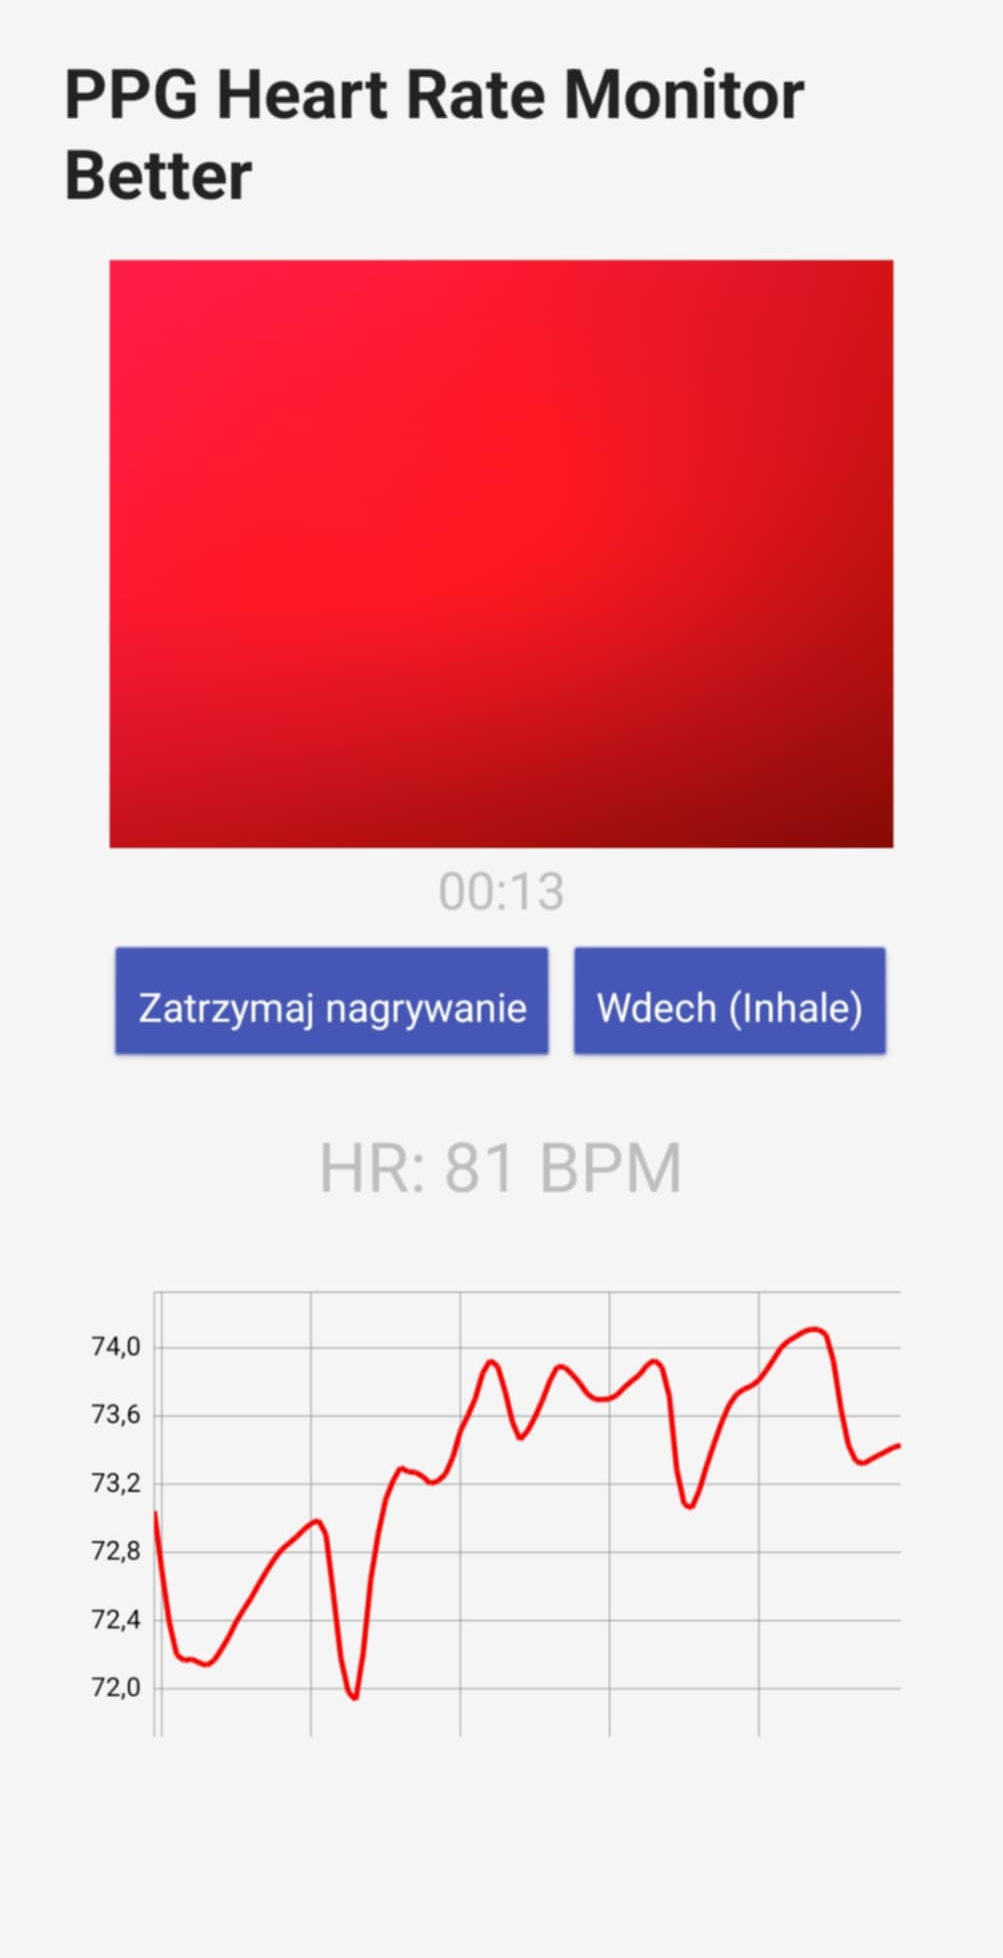
\includegraphics[scale=0.17]{aplikacja.png}
    \caption{Mobile app interface}
    \label{fig:aplikacja_mobilna}
\end{figure}


The application presents the PPG measurements in real time in the form of a dynamicly changing heart rate chart. Registered timestamps corresponding to points of inhales and exhales allow for a correlation with a signal in order to perform an analysis of the relation between the breath cycle and its parameters.
%Aplikacja prezentuje przebieg PPG w czasie rzeczywistym w postaci dynamicznego wykresu zmian rytmu serca. Zarejestrowane znaczniki czasowe odpowiadające momentom wdechu i wydechu umożliwiają korelację z sygnałem w celu analizy zależności między cyklem oddechowym a jego parametrami.


Registered record is subject to a low-pass filter. Lokal maximums detection is realised by analysing three consecutive signal samples. The middle point is classified as a peak if its vvalue exceeds the value of the neighbouring points. Acknowleding a new peak requires for a timespan of at least 600 ms from the previous peak which reduces erroneous identifications resulting from movement interferences. Extremum identification is registered in conjunction with the timestamp and used to dynamicaly compute the Beats Per Minute as per the equation (1) :
%Zarejestrowany zapis ulega filtracji dolnoprzepustowej. Detekcja lokalnych maksimów realizowana jest poprzez analizę trzech kolejnych próbek sygnału, środkowy punkt klasyfikowany jest jako szczyt, jeśli jego wartość przewyższa oba sąsiednie. Akceptacja następnego piku wymagana upływu co najmniej 600 ms od poprzedniego wykrycia, ograniczając błędne rozpoznania wynikające z zakłóceń ruchowych. Zidentyfikowane ekstremum jest rejestrowane wraz ze znacznikiem czasu i wykorzystywane do dynamicznego wyznaczania częstości uderzeń serca BPM, zgodnie z równaniem (1) :

\begin{equation}
\text{BPM} = \frac{60}{\Delta t}
\label{eq:bpm}
\end{equation}
where $\Delta t$  - average timespan between consecutive signal peaks

%Opracowana aplikacja mobilna została udostępniona publicznie pod adresem:
The source code of the developed mobile application has been hosted at the address:
\href{https://github.com/JanBancerewicz/PPGbetter}{GitHub – Aplikacja PPG}

\newpage
%Proces rejestracji sygnału
\paragraph{Signal recording method}
Data used to train and validate wave peak detection model has been acquired using the developed application. Images were captured in real time in YUV 4:2:0 format at 640×480 resolution. An average brightness pixel value was being computed based on a lumination component isolated isolated from every frame. The reulst of the computation represents a single sample of raw photoplethysmographic signal.
%Dane wykorzystane do trenowania i walidacji modelu detekcji szczytów fali zostały pozyskane przy użyciu zaprojektowanej aplikacji. Obrazy przechwytywano w czasie rzeczywistym w formacie YUV 4:2:0 o rozdzielczości 640×480. Z każdej klatki wyodrębniano składową luminancji, na podstawie której obliczano średnią wartość jasności pikseli. Otrzymany odczyt stanowił pojedynczą próbkę surowego sygnału fotopletyzmograficznego.

A series of measurements with the participation of six people has been performed in order to gather the necessery amount of data. Every session lasted 10 minutes and involved registration of the signal in varied condidions taking small finger movement into account.
%W celu zgromadzenia odpowiedniego zbioru danych zrealizowano serię pomiarów z udziałem sześciu osób. Każda sesja trwała 10 minut i obejmowała rejestrację sygnału w zróżnicowanych warunkach, uwzględniających drobne ruchy palca wpływające na zmienność przepływu krwi.

Transmission of data between the smartphone and the server has been performed using the WebSocket protocol. Data was sent in packets containing single measurement points along with their corresponding timestamps. Sampling frequency was consistent with the number of frames per second which totaled about 30 Hz. Received data was buffered on the server and saved in CSV format.
% Transmisję danych pomiędzy smartfonem a komputerem przeprowadzono z wykorzystaniem protokołu WebSocket. Informacje przesyłano w pakietach zawierających pojedyncze punkty pomiarowe wraz z odpowiadającymi im znacznikami czasu. Częstotliwość próbkowania była zgodna z liczbą klatek wideo, wynoszącą około 30 Hz. Odebrane dane buforowano na komputerze i zapisywano w formacie CSV.

%Filtracja sygnału – filtr Butterwortha
% TODO:(mati): first sentence - double check
% TODO:(mati): monotoniczne tłumienie, zbocze przejściowe
\subsection{Signal filtration - Butterworth filter}
Butterworth has been developed as an analogue solution with a maximally flat amplitude characteristic in the band-pass, minimizing the oscillations and signal distortions. It is characterised by monotonic suppression in the stopband and a milder transitional slope then in higher selectivity structures like Czebyszev and eliptic \cite{22}. In the digital implementation it takes the form of a system with an Infinite Impulse Response where the given output sample depends on the both input values as well as previous output values. This approach enables deployment of higher order filters given a limited coefficient count used in real time applications \cite{23}.
%Filtr Butterwortha opracowano jako rozwiązanie analogowe o maksymalnie płaskiej charakterystyce amplitudowej w paśmie przepustowym, minimalizującej oscylacje i zniekształcenia sygnału. Charakteryzuje się monotonicznym tłumieniem w paśmie zaporowym oraz łagodniejszym zboczem przejściowym niż w strukturach o wyższej selektywności, w tym Czebyszewa i eliptycznych \cite{22}. W implementacji cyfrowej przyjmuje postać układu o nieskończonej odpowiedzi impulsowej IIR, gdzie bieżąca próbka wyjściowa zależy od wartości wejściowych, jak i poprzednich stanów wyjściowych. Podejście to umożliwia realizację filtrów wyższych rzędów przy ograniczonej liczbie współczynników, wykorzystywanych w aplikacjach czasu rzeczywistego \cite{23}.

\begin{figure}[htbp]
    \centering
    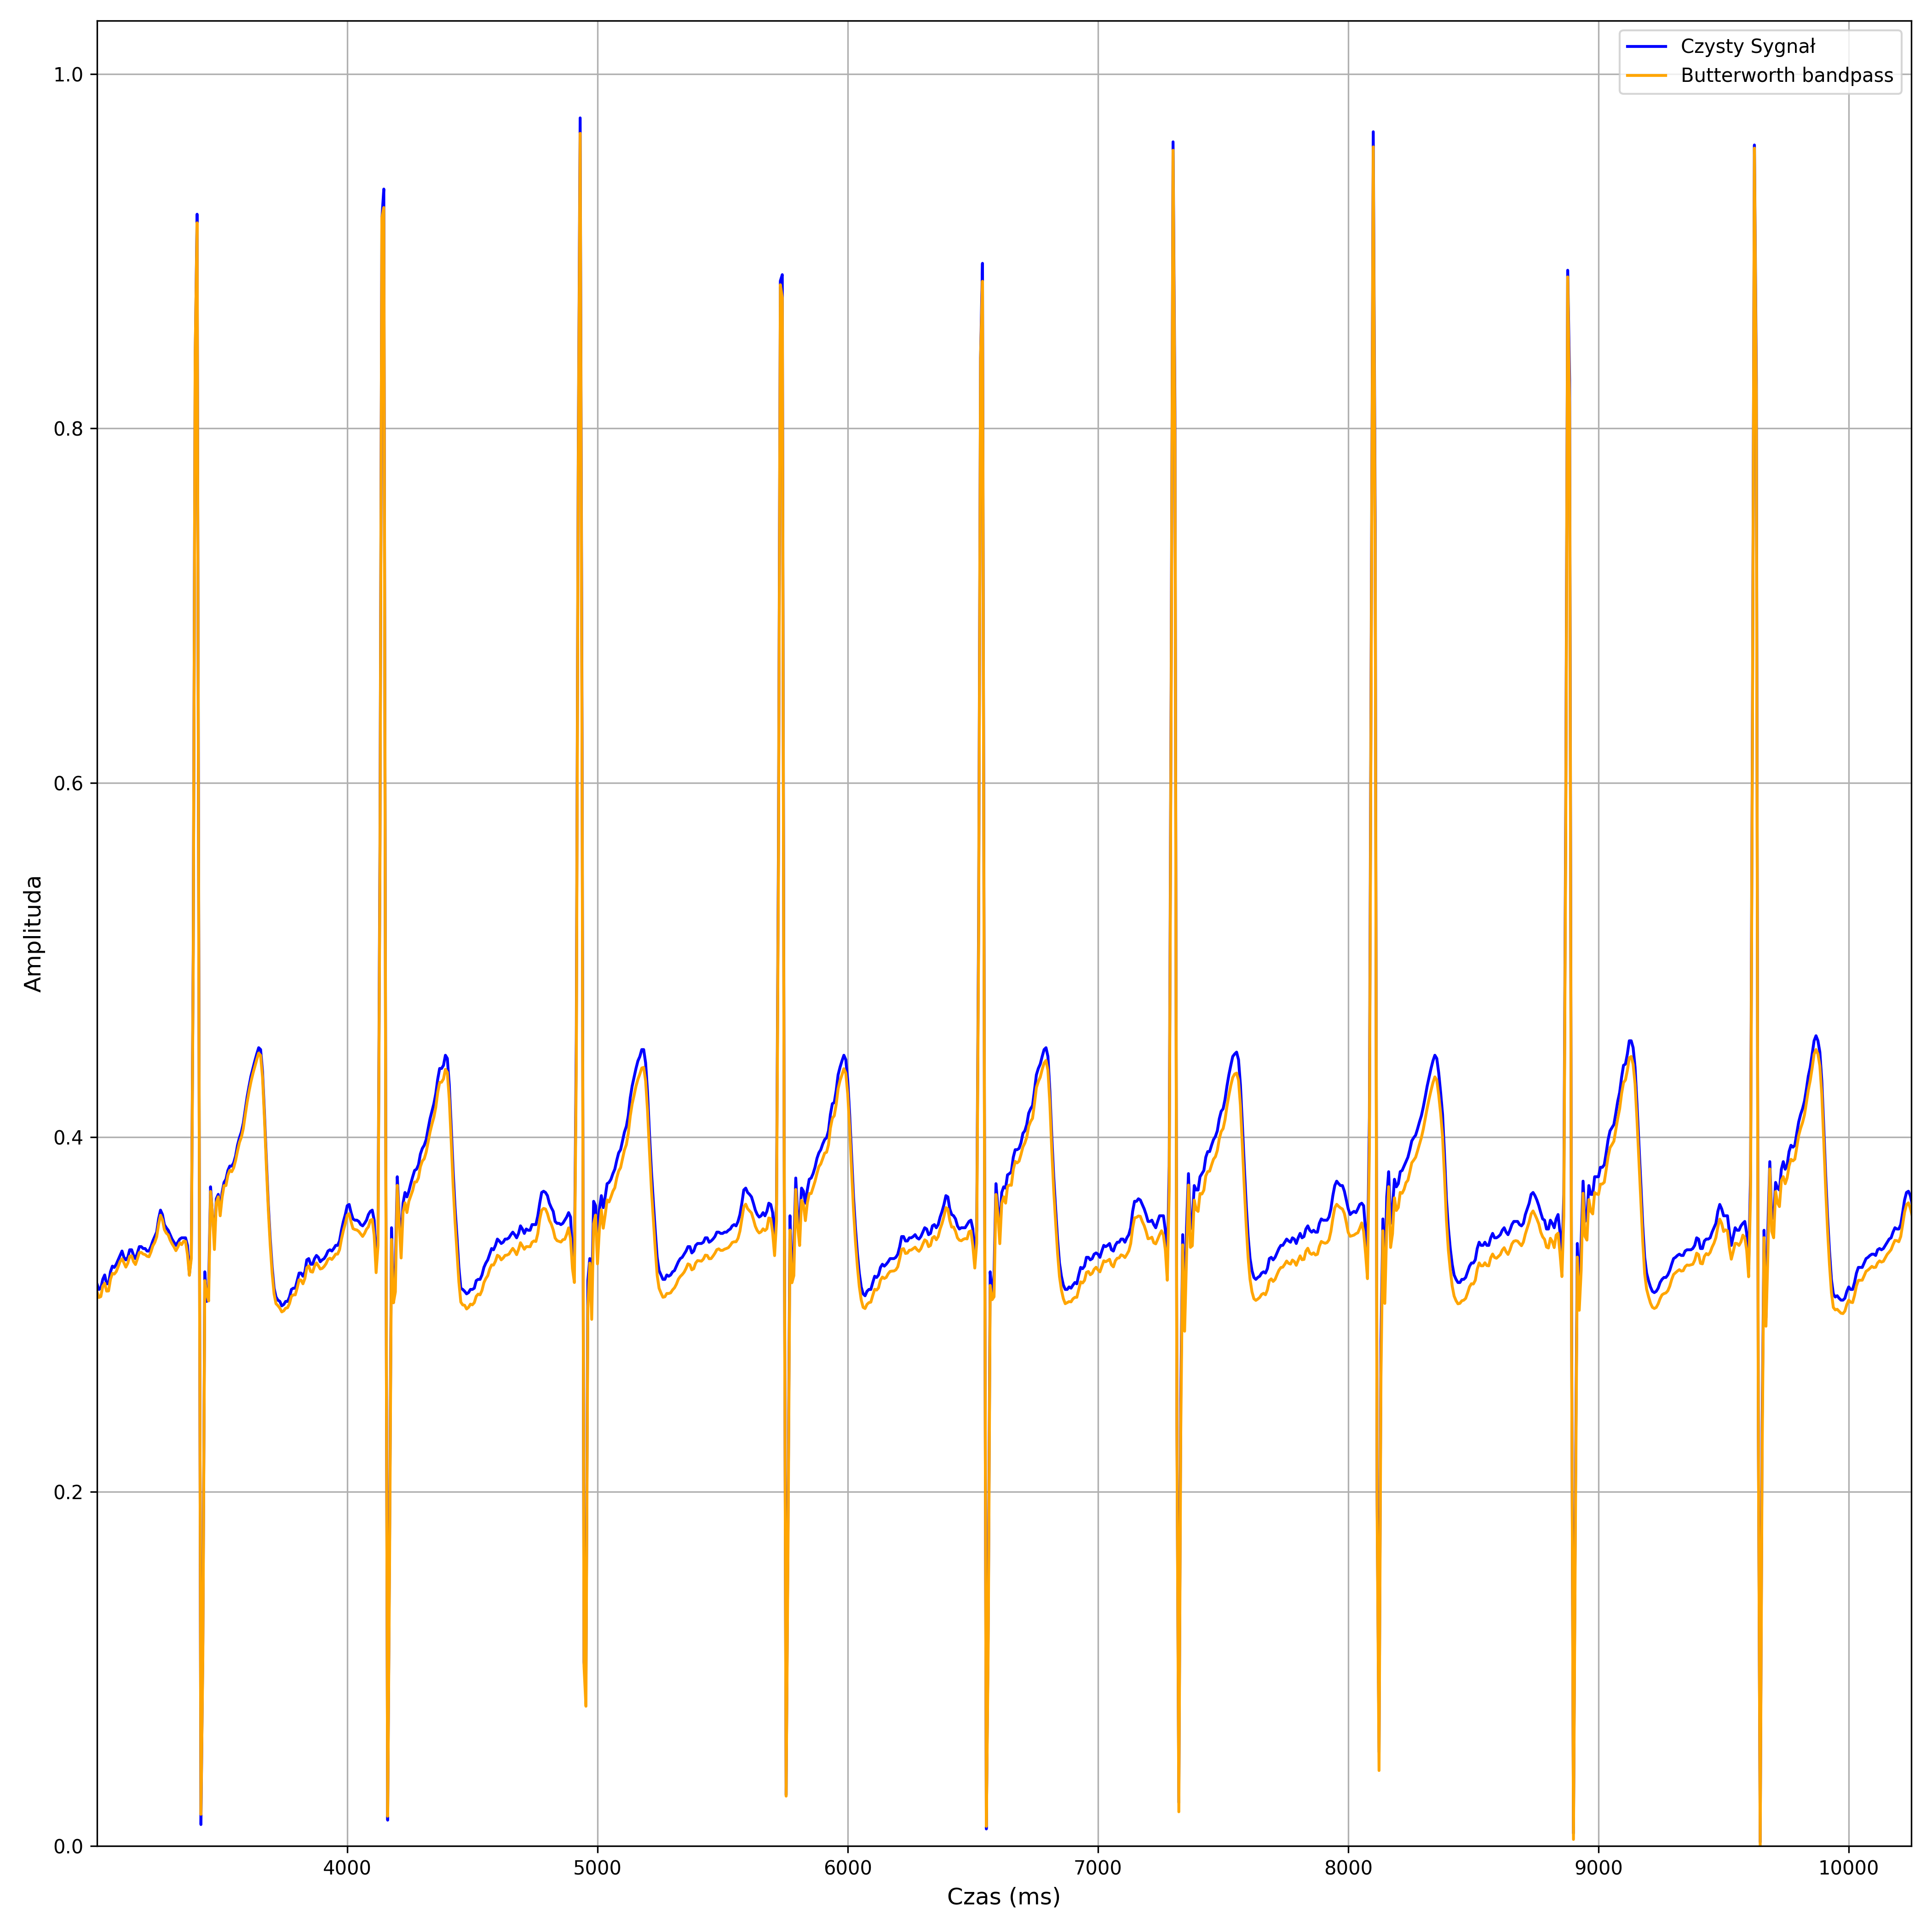
\includegraphics[width=0.76\linewidth]{Filtr_EKG.png} 
    \caption{A comparison between raw and filtered ECG signals}
    \label{fig:filtr_ekg}
\end{figure}

A fifth order digital filter is used to process ECG signal. The filter has a passband characteristic with a frequency range of 0.5 Hz to 45 Hz. The filter eliminates both noise as well as interferences. The lower band limit reduces the slow changes in the record caused by body movement or instable electrodes position \cite{24}. The upper limit on the other hand suppresses network, electromagnetic and muscle interferences \cite{25}. Data filtration as been performed based on the NeuroKit2 library.
%Do przetwarzania sygnału EKG wykorzystano cyfrowy filtr piątego rzędu o charakterystyce pasmowo-przepustowej, obejmującej zakres częstotliwości od 0,5 Hz do 45 Hz, eliminujący szumy oraz zakłócenia. Dolna granica pasma redukuje powolne zmiany w zapisie wywołane ruchem ciała lub niestabliną pozycją elektrod  \cite{24}. Natomiast górna tłumi zakłócenia sieciowe, elektromagnetyczne oraz mięśniowe  \cite{25}. Filtracja danych została przeprowadzona w oparciu o bibliotekę NeuroKit2.


\begin{figure}[htbp]
    \centering
    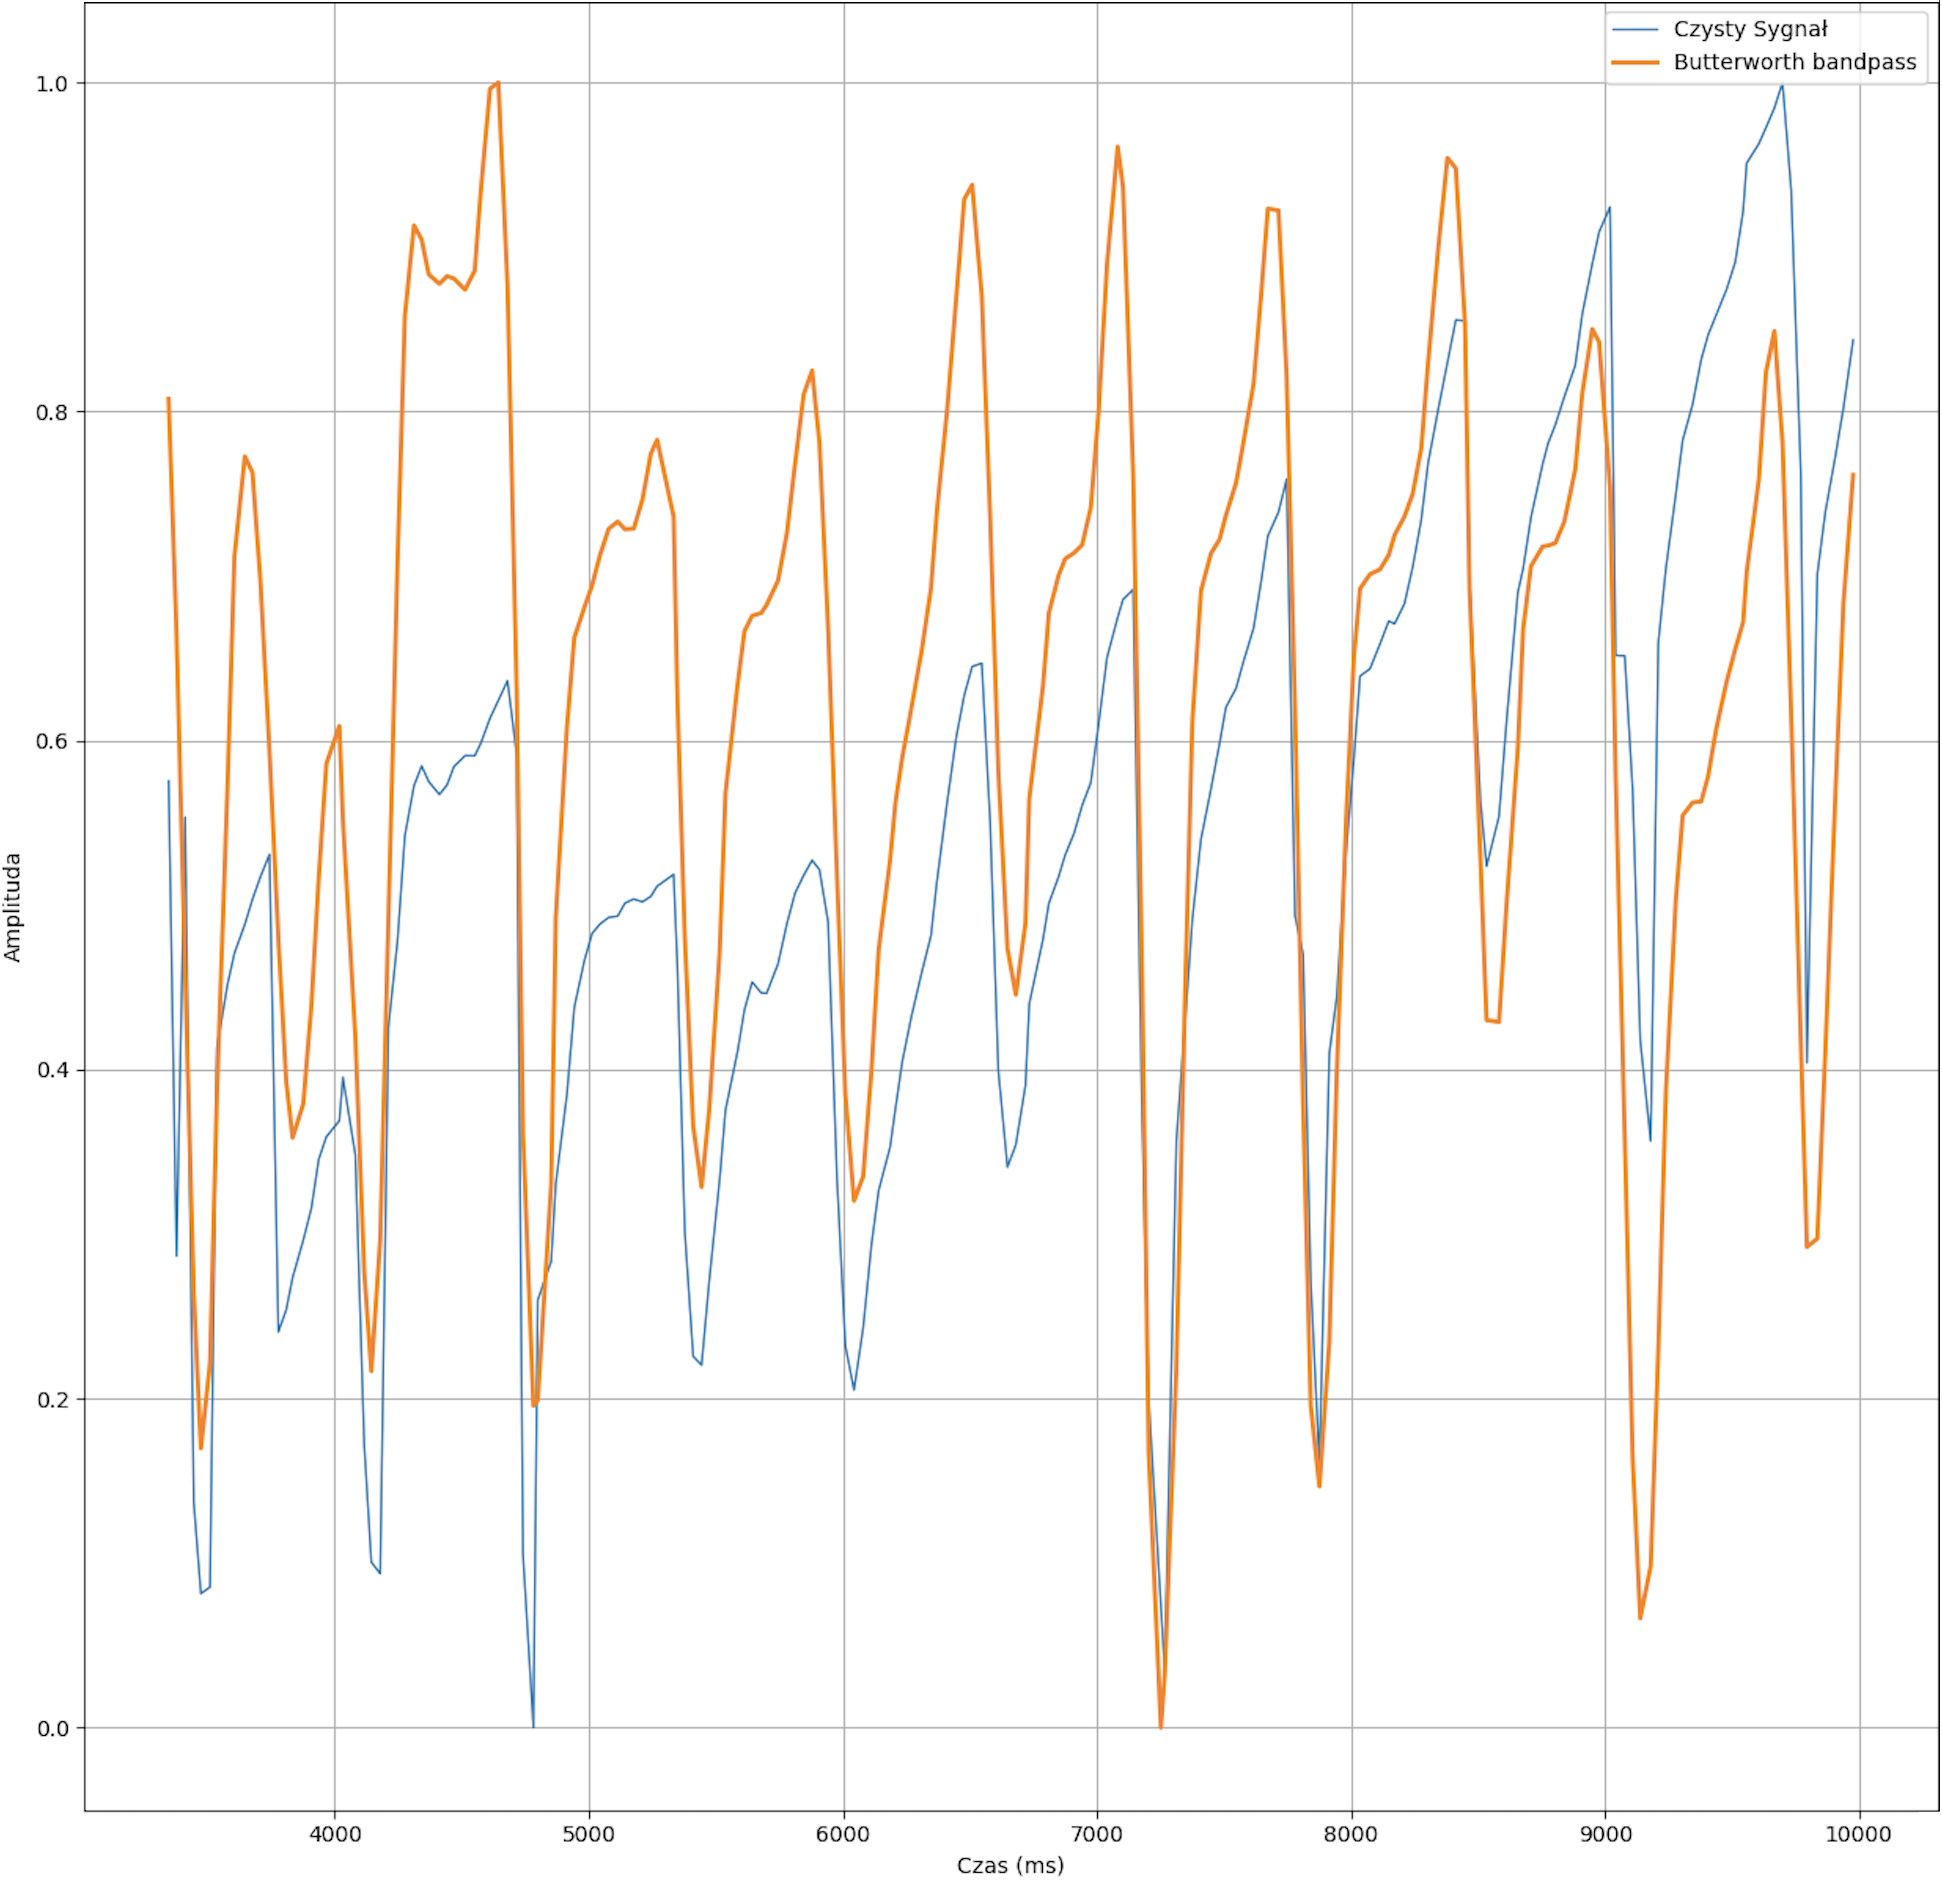
\includegraphics[width=0.76\linewidth]{Filtr_PPG.png} 
    \caption{A comparison between raw and filtered PPG signal}
    \label{fig:filtr_ppg}
\end{figure}

To improve the PPG signal quality a fourth order filter with the working range of 0.5-5 Hz has been employed. The lower band limit reduces the interferences caused by body movements or instable position of the detector. The upper limit suppresses the measuring device noise and optical interferences \cite{26}. Filtration has been implemented by using the SciPy module to prevent phase shifts of the measurement.
%Dla poprawy jakości sygnału PPG wykorzystano filtr  czwartego rzędu, działający w zakresie 0,5–5 Hz. Dolna granica pasma ogranicza zakłócenia spowodowane ruchem ciała czy niestabilnym kontaktem czujnika ze skórą, natomiast górna tłumi szumy urządzenia pomiarowego i interferencje optyczne  \cite{26}. Filtracja została zrealizowana z wykorzystaniem  modułu SciPy, zapewniając obróbkę przebiegu bez przesunięcia fazowego.

%Modele detekcji
% Model do wykrywania załamków R
\newpage
\subsection{Detection models}
\subsubsection{R peak detection model}
A neural network combining convolutional and recursive layer has been developed. Its purpose is R peak detection in ECG record. The network constitutes the first step in computing the RR intervals and computing the heart rate variability parameters. The model processes one-dimensional electric-voltage signals divided into fragment. Each fragment contains 256 samples and is a basic unit of measurement analysis.
% Opracowano sieć neuronową łączącą warstwy splotowe i rekurencyjne, przeznaczoną do detekcji szczytów R w zapisie EKG. Stanowi ona pierwszy etap w wyznaczaniu interwałów RR i obliczaniu parametrów zmienności rytmu serca. Model przetwarza jednowymiarowe sygnały napięcia elektrycznego podzielone na fragmenty po 256 próbek, stanowiących podstawową jednostkę analizowanego przebiegu.

Convolutional portion of the network is comprised of four 1D convolutional layers, parameters of which have been presented in a Chart~\ref{tab:ecg_layers}. Those layers are responsible for extracting the features from the input signal and extending its representation by increasing the number of channels from 16 to 256 using 3 and 5 order filters. For each transformation BatchNorm1d normalisation and nonlinear activation function LeakyReLU have been applied. Dimension count reduction is realized using a MaxPooling1D operation with a core size of 2 which shortens the sequence from 256 to 16 samples along the time axis and increasing the model's resistance to noise and interference. The output [128 × 16] matrix is the input for a one-way LSTM. The resulting vector is flattened and given to a layer with 128 neurons. In the next step the result is fit into a final block with 256 elements each representing subsequent input signal samples. Output data from LSTM layer are processed by linear modules propagating extracted features into logit space. Every element of the vector corresponds to a probability of a R peak in the given sample allowing for a binary classification in every point in the measurement.
% Część splotowa sieci obejmuje cztery warstwy konwolucyjne 1D, których parametry zestawiono w Tabeli~\ref{tab:ecg_layers}. Warstwy te odpowiadają za ekstrakcję cech z sygnału wejściowego, rozszerzając jego reprezentację poprzez zwiększenie liczby kanałów od 16 do 128 za pomocą filtrów o rozmiarach 5 i 3. Dla każdego przekształcenia zastosowano normalizację BatchNorm1d oraz nieliniową funkcję aktywacji LeakyReLU. Redukcja wymiarowości jest realizowana za pomocą operacji MaxPooling1D z jądrem o rozmiarze 2, skracającej długość sekwencji z 256 do 16 próbek wzdłuż osi czasowej oraz zwiększającej odporność modelu na szum i zakłócenia. Wynikowa macierz o wymiarach [128 × 16] stanowi wejście dla jednokierunkowej LSTM. Otrzymany wektor jest spłaszczany i przekazywany do warstwy z 128 neuronami, a następnie do bloku końcowego zawierającego 256 elementów, reprezentujące kolejne próbki sygnału wejściowego. Dane wyjściowe z warstwy LSTM są  przetwarzane przez moduły liniowe, odwzorowujące wyekstrahowane cechy w przestrzeń logitów. Każdy element wektora odpowiada prawdopodobieństwu obecności szczytu R w danej próbce, umożliwiając binarną klasyfikację w każdym punkcie czasowym przebiegu. 

%Parametry bloków konwolucyjnych sieci
\begin{table}[h!]
\centering
\caption{Block parameters of convolutional networks}
\label{tab:ecg_layers}
\begin{tabular}{|l|c|c|c|c|c|}
\hline
\textbf{Block} & \textbf{In.} & \textbf{Out.} & \textbf{Filter} & \textbf{Padding} & \textbf{Act./Norm.} \\
\hline
Conv1D-1 & 1   & 16  & 5 & 2 & LReLU+BN \\
Conv1D-2 & 16  & 32  & 5 & 2 & LReLU+BN \\
Conv1D-3 & 32  & 64  & 3 & 1 & LReLU+BN \\
Conv1D-4 & 64  & 128 & 3 & 1 & LReLU+BN \\
\hline
\end{tabular}
\end{table}

Model has been trained in a supervised mode based on the signals acquired from Polar H10 detector. Actual R peaks in a filtered ECG record have been computed using the Pan-Tompkins algorithm based on multistep processing. The first phase is band-pass suppression of low and high frequency distortionary components. Measurement differentiation enhances steep curves of QRS complex. Afterwords a square of an average value of all samples in a moving integrating window is being computed. The final peak detection is realized through propagating the integrated curve and local maximums analysis \cite{27}.
Every point is assigned a binary label identifying the presence or lack thereof of an extremum. This allows for a pattern classification corresponding to acrtual R peaks.
\newpage
Learning process has been performed in series of 32 elements using the BCEWithLogitsLoss loss function. Adam algorithm was used to optimize with a constant learning rate of 0.0001. The efficiency of the developed neural network has been assessed based on the results obtained from an independant dataset using the model's trained parameters. Classification results have been presented in the form of a confusion matriz in Chart~\ref{tab:conf_matrix}.
%Model wytrenowano w trybie nadzorowanym na podstawie sygnałów pozyskanych z czujnika Polar H10. Rzeczywiste załamki R w przefiltrowanym zapisie EKG wyznaczono algorytmem Pan–Tompkinsa opartym na wieloetapowym przetwarzaniu. Początkową fazą jest pasmowo-przepustowe tłumienie składowych zakłócających o niskiej oraz wysokiej częstotliwości. Różniczkowanie przebiegu uwydatnia strome zbocza zespołu QRS, następnie obliczana jest średnia wartość próbek podniesionych do kwadratu w ruchomym oknie całkującym. Ostateczna detekcja szczytów jest realizowana poprzez progowanie zintegrowanej krzywej oraz analizę lokalnych maksimów \cite{27}.
%Każdemu punktowi przypisano etykietę binarną wskazującą obecność lub brak ekstremum, umożliwiając sieci klasyfikację wzorców odpowiadających rzeczywistym pikom R. 
%\newpage
%Proces uczenia przeprowadzono w partiach po 32 elementy z wykorzystaniem funkcji straty BCEWithLogitsLoss. Do optymalizacji zastosowano algorytm Adam przy stałej wartości learning rate wynoszącej 0,0001. Efektywność zaprojektowanej sieci neuronowej oceniono na podstawie wyników uzyskanych na niezależnym zbiorze danych, wykorzystując wytrenowane parametry modelu. Rezultaty klasyfikacji przedstawiono w postaci macierzy konfuzji w Tabeli~\ref{tab:conf_matrix}.


\begin{table}[ht]
\centering
\caption{Confusion matrix for R peak detection}
\label{tab:conf_matrix}
\begin{tabular}{|c|c|c|}
\hline
\textbf{Actual / Prediction} & \textbf{No peak } & \textbf{Peak } \\
\hline
No peak  & 231170 & 53 \\
Peak  & 83 & 2678 \\
\hline
\end{tabular}
\end{table}

231170 samples not containing the R peak and 2678 with its actual pressence have been correctly classified by the model. The number of false positive prediction totaled 53 while the  nnumber of false negatives -- 83. The value of the F1 benchmark being equal to 0.9753 attests to a balanse between precision and sensitivity of the model, a key feature of automated electrocardiographical signal analysis. Basic quality assessment metrics have been presented in Chart~\ref{tab:metrics}.
%Model poprawnie zaklasyfikował 231170 próbek niezawierających piku R oraz 2678 z jego rzeczywistą obecnością. Liczba fałszywie pozytywnych predykcji wyniosła 53, natomiast fałszywie negatywnych -- 83. Wartość miary F1 równa 0,9753 świadczy o wysokiej równowadze pomiędzy precyzją a czułością modelu, co jest kluczowe w automatycznej analizie sygnałów elektrokardiograficznych. Podstawowe metryki oceny jakości modelu przedstawiono w Tabeli~\ref{tab:metrics}.

\begin{table}[ht]
\centering
\caption{R peak detection parameters}
\label{tab:metrics}
\begin{tabular}{|c|c|p{4.6cm}|}
\hline
\textbf{Metric} & \textbf{Value} & \textbf{Description} \\
\hline
Efficiency & 96,99\% & A percentage of correct classifications of R peaks or lack thereof. \\
Incorrect detections & 0,00\% & A percentage of samples falsely classified as containing R peaks. \\
Skipped peaks & 3,01\% & A percentage of samples with undetected actual R peaks. \\
\hline
\end{tabular}
\end{table}

%Model do wykrywania szczytów fali
\subsubsection{Wave peak detection model}
Analogously to the approach applied in the ECG signal analisys a convolutional model identifing local peaks in photoplethysmographic measurement has been developed. The model constitutes a base to determining Inter Beat Intervals used to estimate heart rate indicators. The network processes the data in the form o f a vector containing 50 samples in a single channel. Those samples represent changes of the blood volume in the vessels.
%Analogicznie do podejścia zastosowanego w analizie sygnału EKG, opracowano model konwolucyjny identyfikujący lokalne szczyty w przebiegu fotopletyzmograficznym. Stanowi on podstawę do wyznaczania interwałów międzyuderzeniowych IBI, wykorzystywanych przy estymacji wskaźników rytmu serca. Sieć przetwarza dane w postaci wektora zawierającego 50 próbek w pojedynczym kanale, reprezentujących zmiany objętości krwi w naczyniach obwodowych.

A one-dimensional convolutional layer with 32 filters each the width of 7 samples complemented with BatchNorm1d normalisation and activation function GELU constitutes the first element of the architecture. The activation function's purpose is increasing the stability of the learning process and gentle non-linearity. The next four residiual blocks process the local signal patterns. The first module increases the number of channels from 32 to 64 utilizing a core with a size of 9. Extending the number of dimensions from 64 to 128 is realized by the next segment using a 5 sample wide window. The remaining two modules maintain the same depth while operating with filters with sizes of 3 and 7 repsectively. Transformations defined in the beggining stage have been extended with a Dropout layer ensuring a reduction in overfitting.
\newpage
The SE module raises the model's selectivity which improves the accuracy of detectig local measurement maximums. A convolutional block with a size of 1 core compresses the number of channels from 128 to 64 while two fully connected linear operations reduce the number of dimensions to 64 and 32 including the GELU activation function. A one-dimensional output vector is subject to a Sigmoid transformation allowing for intepreting the vales as probabilities of local peaks in PPG record. Detailed block parameters have been included in a Chart~\ref{tab:ppg_layers}.
%Pierwszy element architektury stanowi jednowymiarowa warstwa splotowa z 32 filtrami o szerokości 7 próbek, uzupełniona normalizacją BatchNorm1d oraz funkcją aktywacji GELU, odpowiedzialną za łagodną nieliniowość i poprawę stabilność procesu uczenia. Cztery kolejne bloki resztkowe przetwarzają lokalne wzorce sygnału. Pierwszy moduł zwiększa kanały z 32 do 64, wykorzystując jądro o rozmiarze 9.  Rozszerzenie liczby wymiarów z 64 do 128 realizuje segment przy zastosowaniu okna o długości 5 próbek, natomiast dwa pozostałe utrzymują tę samą głębokość, operując filtrami o wielkości 3 i 7. Transformacje zdefiniowane w początkowym etapie zostały rozszerzone o warstwę Dropout, umożliwiającą redukcję nadmiernego dopasowania. 
%\newpage
%Moduł SE podnosi selektywność modelu, poprawiając precyzję wykrywania lokalnych maksimów przebiegu. Kompresję kanałów z 128 do 64 zapewnia blok konwolucyjny z jądrem o rozmiarze 1, a dwie w pełni połączone operacje liniowe zmniejszają wymiary do 64 i 32, z funkcją aktywacji GELU. Jednowymiarowy wektor wyjściowy podlega transformacji Sigmoid, umożliwiając interpretację wartości jako prawdopodobieństwo lokalnych szczytów w zapisie PPG. Szczegółowe parametry bloków uwzględniono w Tabeli~\ref{tab:ppg_layers}.

%Parametry bloków konwolucyjnych sieci
\begin{table}[ht]
\centering
\caption{Convolutional network's block parameters}
\label{tab:ppg_layers}
\begin{tabular}{|l|c|c|c|c|c|}
\hline
\textbf{Block} & \textbf{In.} & \textbf{Out.} & \textbf{Filter} & \textbf{Padding} & \textbf{Act./Norm.} \\
\hline
Conv1D & 1 & 32 & 7 & 3 & GELU+BN \\
ResidualBlock 1 & 32 & 64 & 9 & 4 & GELU+BN+DO \\
ResidualBlock 2 & 64 & 128 & 5 & 2 & GELU+BN+DO \\
ResidualBlock 3 & 128 & 128 & 3 & 1 & GELU+BN+DO\\
ResidualBlock 4 & 128 & 128 & 7 & 3 & GELU+BN+DO \\
SEBlock & 128 & 128 & – & – & SE scaling \\
Conv1D  & 128 & 64 & 1 & 0 & GELU+BN \\
FC & 128 & 64 & – & – & GELU \\
FC & 64 & 32 & – & – & GELU \\
Output & 32 & 1 & – & – & Sigmoid \\
\hline
\end{tabular}
\end{table}

The process of superviesed learning for PPG data has been performed for signal segments originating from a mobile device, subject to preliminary filtration and normalisation to [-1, 1] range. Every segment has been assigned a vector of binary labels signifying a peak or lack thereof. The vector is based on a local peak identification which exceed their neighbouring values allowing for classification in the range of the window. The networks was trained on 50-point measurement fragments in series of 32 segments utilizing BCELoss function and Adam optimizer with a constant learning rate of 0.001. The efficiency of the developed model has been assessed based on the results acquired from an independent dataset using the parameters determined during the fitting. Classification results have been presented in the form of a confusion matrix in a Chart~\ref{tab:conf_matrix_ppg}.
%Proces uczenia nadzorowanego dla danych PPG przeprowadzono na segmentach sygnału pochodzących z urządzenia mobilnego, poddanych wstępnej filtracji i normalizacji do zakresu [-1, 1]. W każdym wycinku przypisano wektor etykiet binarnych określający obecność lub brak piku, oparty na identyfikacji lokalnych szczytów przewyższających sąsiednie wartości, umożliwiając klasyfikację wzorców w obrębie okna. Sieć trenowano na 50-punktowych fragmentach przebiegu, w partiach po 32 segmenty, wykorzystując funkcję straty BCELoss oraz optymalizator Adam ze stałym współczynnikiem uczenia równym 0,001. Skuteczność zaprojektowanego modelu oceniono na podstawie wyników uzyskanych na niezależnym zbiorze danych, przy zastosowaniu parametrów wyznaczonych podczas dopasowania. Wyniki klasyfikacji przedstawiono w formie macierzy konfuzji w Tabeli~\ref{tab:conf_matrix_ppg}.

%Macierz konfuzji dla detekcji pików fali
\begin{table}[ht]
\centering
\caption{Confusion matrx for wave peaks detection}
\label{tab:conf_matrix_ppg}
\begin{tabular}{|c|c|c|}
\hline
\textbf{Actual / Prediction} & \textbf{No peak } & \textbf{Peak} \\
\hline
No peak  & 9609 & 9 \\

Peak  & 7 & 375 \\
\hline
\end{tabular}
\end{table}

% TODO:(mati): miara F1 -> F1 benchmark?
For photoplethysmographic signals the network has correctly identified 375 samples containing the wave peak and 9609 samples without one. Incorrect predictions have been noted in 9 falsely positive and 7 falsely negative cases. The obtained value 0.9774 of the F1 benchmark is close to the result of the one from the ECG model confirming the validity of the applied solution in the analysis of both signal types.
Basic quality assessment metrics of the architecture have been presented in a Chart~\ref{tab:metrics_ppg}.
%Dla sygnałów fotopletyzmograficznych sieć poprawnie rozpoznała 9609 próbek bez obecności fali oraz 375 z jej wystąpieniem. Niepoprawne predykcje odnotowano w 9 przypadkach fałszywie dodatnich oraz 7  fałszywie ujemnych. Otrzymana wartość miary F1, wynosząca 0,9774, jest zbliżona do wyników uzyskanych dla modelu EKG, potwierdzając wiarygodność zastosowanego rozwiązania w analizie obu typów sygnałów.
%Podstawowe metryki oceny jakości architektury przedstawiono w Tabeli~\ref{tab:metrics_ppg}.

%Parametry detekcji szczytów fali
\begin{table}[ht]
\centering
\caption{Wave peak detection parameters}
\label{tab:metrics_ppg}
\begin{tabular}{|c|c|p{4.6cm}|}
\hline
\textbf{Metric} & \textbf{Value} & \textbf{Description} \\
\hline
Efficiency & 98,17\% & Percentage of correctly classified samples. \\
Incorrect detections & 0,52\% & Percentage of samples falsely classified as containing the wave peak. \\
Skipped peaks & 1,83\% & Percentage of sample with undetected actual wave peak. \\
\hline
\end{tabular}
\end{table}

%Ewaluacja maksimów i analiza czasowa sygnałów biomedycznych
%Weryfikacja skuteczności detekcji pików R
\newpage
\section{Maximums evaluation and time analysis of biomedical signals}
\subsection{R peak detection efficiency verification}
The efficiency of the architecture based on a convolutional network in R peak detection in electrocardiografical record has been assesed in relation to the classic Pan-Tompkins algorithm and refrencial R peaks acquired using the NeuroKit library which serves as a golden standard. The signal was being samples with the frequency of 130 Hz and processed in misaligned segments covering 256 samples.
%Skuteczność architektury opartej na sieci splotowej w wykrywaniu pików R w zapisie elektrokardiograficznym oceniono względem klasycznego algorytmu Pan–Tompkinsa oraz szczytów referencyjnych uzyskanych w ramach biblioteki NeuroKit, pełniącej rolę złotego standardu. Sygnał próbkowano z częstotliwością 130 Hz i przetwarzano w niepokrywających się segmentach obejmujących 256 próbek. 

The total value of detected maximums reached 54 for the model, 56 using the Pan-Tompkins method and 56 from the referencial data. The results have been presented in a Chart~\ref{tab:peak_comparison}, containing the number of True Positives, False Positives and False Negatives, the computed precision, sensitivity and F1 indicators along with the tolerance corresponding to 1-2 points of the measurement.
% Łączna wartość wykrytych maksimów wyniosła 54 dla modelu, 56 metodą Pan-Tompkinsa oraz 56 w danych wzorcowych. Wyniki przedstawiono w Tabeli~\ref{tab:peak_comparison}, zawierającej liczbę prawdziwych trafień TP, fałszywych alarmów FP, pominiętych szczytów FN, wraz z obliczonymi wskaźnikami precyzji, czułości i F1, przy tolerancji odpowiadającej 1–2 punktom przebiegu.

%Ocena technik wyznaczania ekstremów
\begin{table}[ht]
\caption{Extremums detecting techniques assesment}
\label{tab:peak_comparison}
\centering
\begin{tabular}{|p{3.08cm}|c|c|c|c|c|c|}
\hline
\textbf{Method} & \textbf{TP} & \textbf{FP} & \textbf{FN} & \textbf{Prec.} & \textbf{Sens.} & \textbf{F1} \\
\hline
AI vs Pan-Tompkins & 54 & 0 & 2 & 1.000 & 0.964 & 0.982 \\
AI vs NeuroKit & 53 & 1 & 3 & 0.981 & 0.946 & 0.964 \\
Pan-Tompkins vs NeuroKit & 55 & 1 & 1 & 0.982 & 0.982 & 0.982 \\
\hline
\end{tabular}
\end{table}

\begin{figure}[htbp]
    \centering
    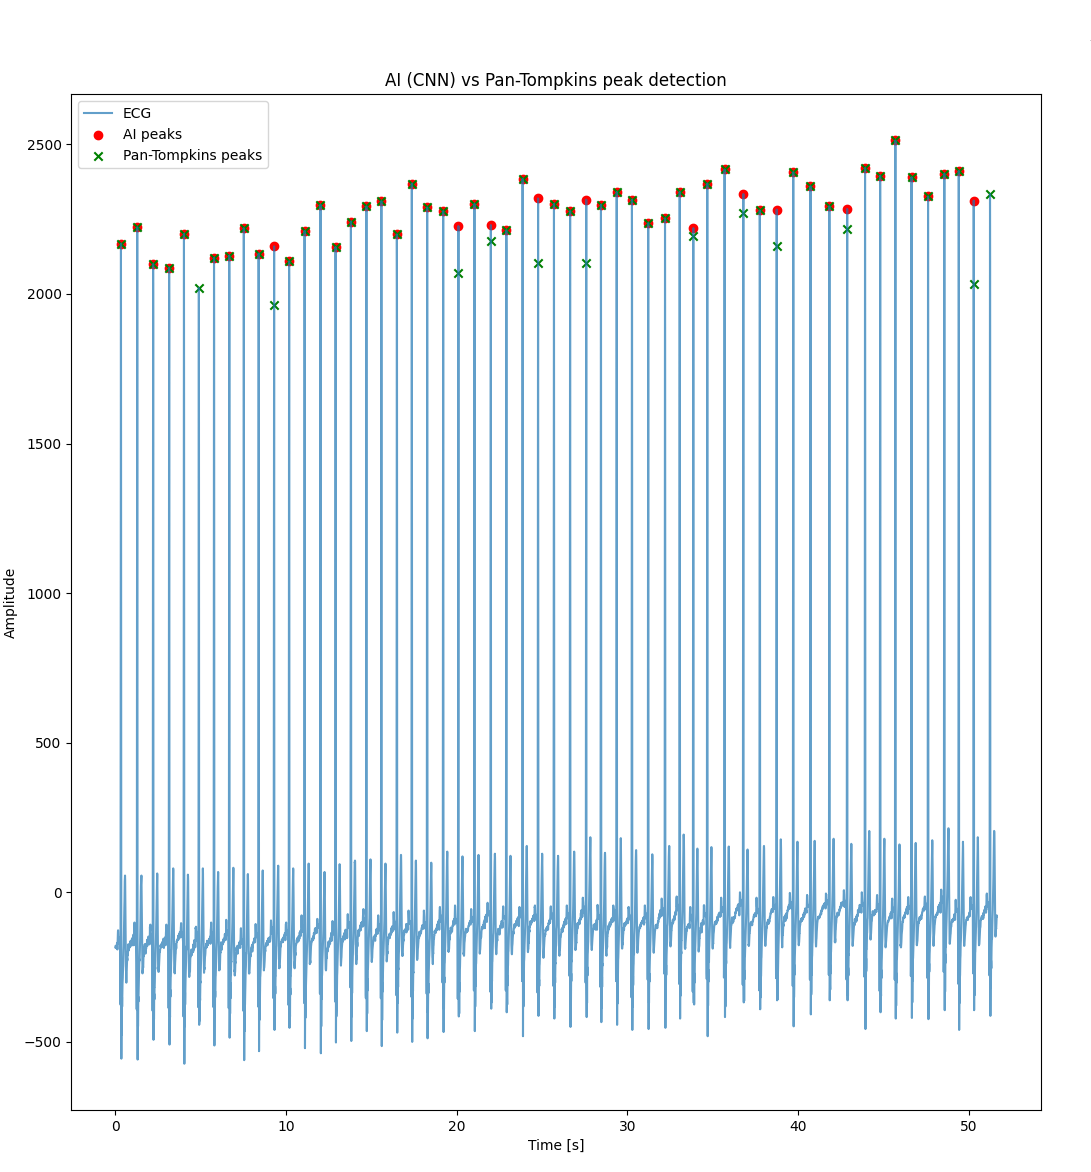
\includegraphics[scale=0.2]{ai_pan-tompkins.png}
    \caption{Comparison of R peak detection between the network and Pan-Tompikns algorithm}
    \label{fig:ai_pan-tompkins}
\end{figure}

\begin{figure}[htbp]
    \centering
    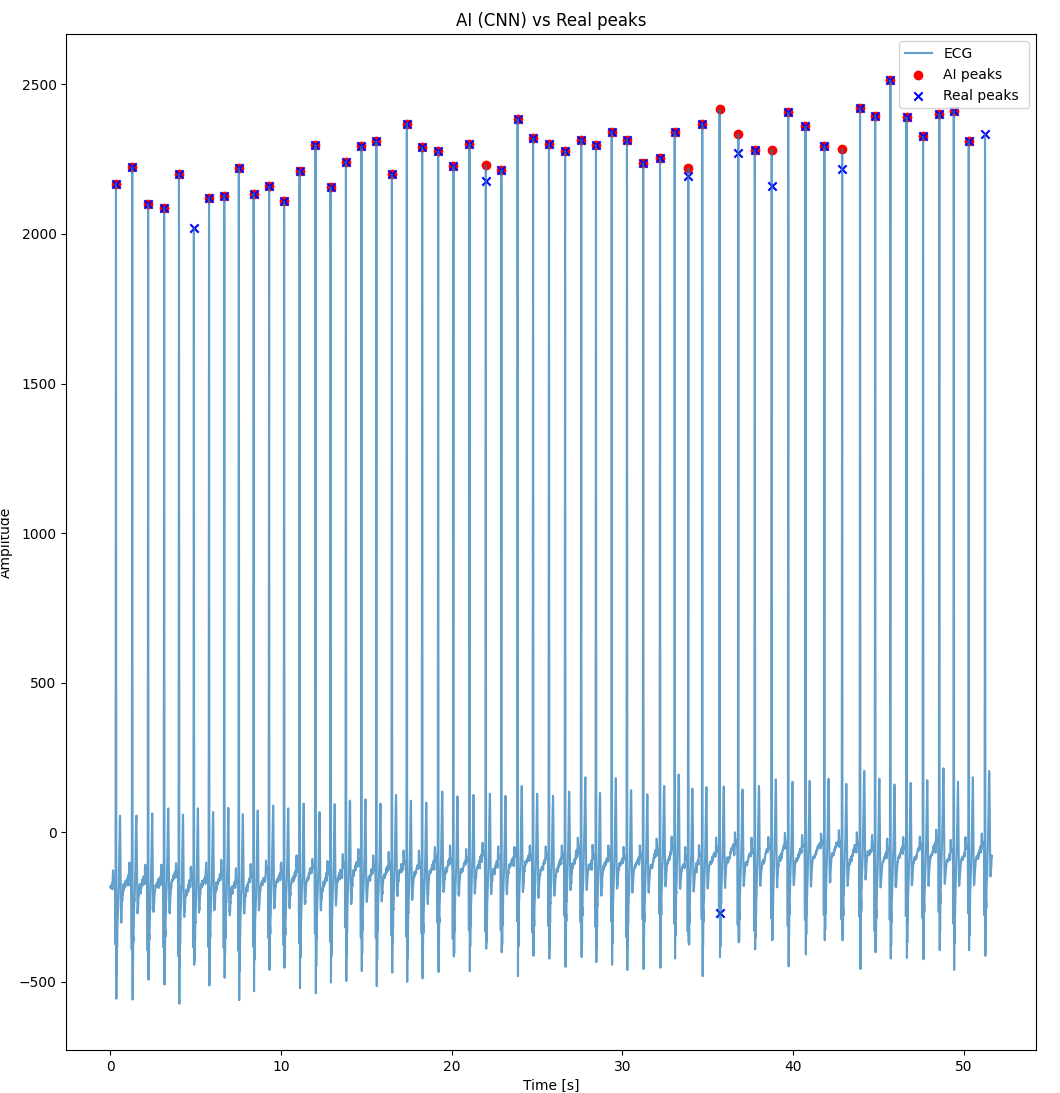
\includegraphics[scale=0.2]{ai_real_peaks.png}
    \caption{Comparison of R peak detection between the network and referencial peaks}
    \label{fig:ai_real_peaks}
\end{figure}


\newpage
Skuteczność sieci w wykrywaniu pików R jest porównywalna z klasycznym algorytmem Pan-Tompkinsa i charakteryzuje się wysoką zgodnością z wartościami referencyjnymi. Rozbieżności wynikające z pominiętych lub przesuniętych ekstremów można zredukować poprzez optymalizację wstępnej obróbki sygnału lub dalsze trenowanie modelu. Obecne systemy uczenia maszynowego wykazują zdolność do osiągania niemal najwyższej klasy skuteczności w automatycznym wykrywaniu lokalnych szczytów zapisu elektrokardiograficznego.

\subsection{Weryfikacja skuteczności detekcji pików fali}
Identyfikacje szczytów przebiegu fotopletyzmograficznego przeprowadzono na podstawie wyników sieci konwolucyjnej oraz sygnału referencyjnego uzyskanego metodą filtracji pasmowo-przepustowej i lokalnego wyszukiwania maksimów. Dane podzielono na segmenty o długości 100 próbek i znormalizowano do zakresu [−1,1]. W trybie okienkowym predykcje modelu przekształcono w indeksy punktów odpowiadających potencjalnym pikom fali.

Algorytm uczenia maszynowego wykrył 76 szczytów, natomiast zestaw wzorcowy obejmował 72. Skuteczność detekcji przebiegła w przedziale tolerancji 264 ms, odpowiadającym 8 jednostkom czasowym przy częstotliwości próbkowania 30 Hz, z zastosowaniem parametrów prawdziwych trafień TP, fałszywych alarmów FP oraz pominiętych pików FN. Model uzyskał 61 TP, 15 FP oraz 11 FN, przekładając się na precyzję 0,803, czułość 0,847 oraz miarę F1 równą 0,824.

\begin{figure}[htbp]
    \centering
    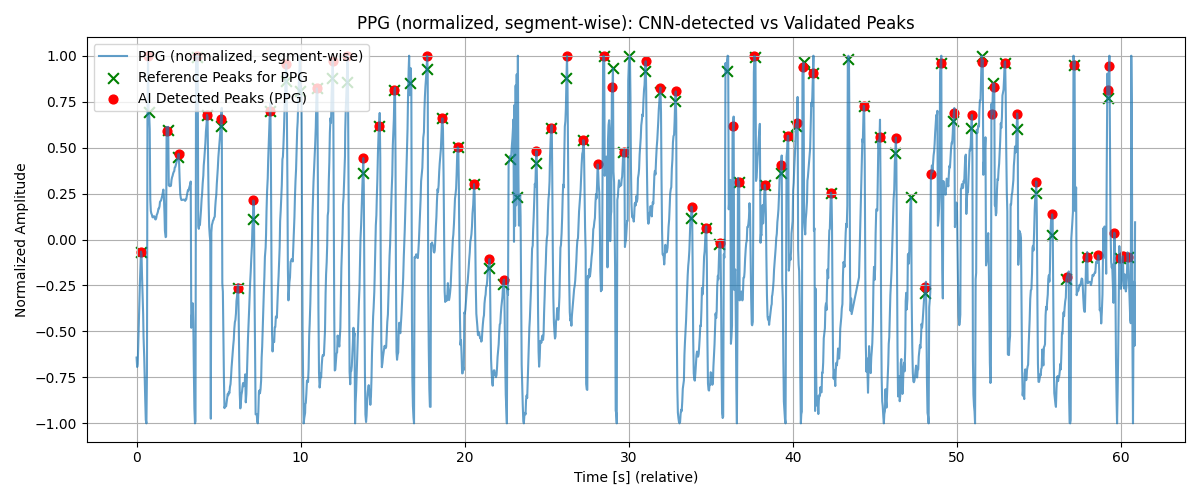
\includegraphics[scale=0.28]{ppg_ai_vs_real.png}
    \caption{Porównanie detekcji pików fali przez sieć splotową z szczytami referencyjnymi}
    \label{fig:ppg_ai_real_peaks}
\end{figure}

\newpage
Wyniki wskazują na wysoką zgodność architektury z referencyjnymi maksimami przebiegu fotopletyzmograficznego, przy niewielkiej liczbie fałszywego wykrywania spowodowanego zakłóceniami i ograniczeniami analizy krótkich segmentów. Uzyskane rezultaty sugerują praktyczną użyteczność sieci w cyfrowym przetwarzaniu sygnałów biomedycznych.


\subsection{Estymacja PTT ze zsynchronizowanych sygnałów}
Podczas rejestracji sygnałów EKG i PPG wykorzystywane są różne schematy zapisu znaczników czasowych. W elektrokardiogramie punkty wystąpienia załamków R początkowo określane są względem chwili rozpoczęcia akwizycji i zapisywane w sekundach jako czas względny. Podczas przetwarzania danych wartości te są przekształcane do formatu absolutnego UNIX, umożliwiając porównanie z przebiegiem PPG. W fotopletyzmografii detekcja szczytów fali rejestrowana jest bezpośrednio w czasie systemowym.

Dla ujednolicenia układu czasowego przekształca się dane EKG z czasu względnego na znaczniki UNIX, zgodnie z równaniem (2):
\begin{equation}
t_{\mathrm{UNIX}} = t_{\mathrm{rel}} + t_{0},
\end{equation}
gdzie $t_{\mathrm{UNIX}}$ - czas w formacie UNIX, $t_{\mathrm{rel}}$ – czas względny, a $t_{0}$ – początek akwizycji.

Przebiegi zostały przedstawione w jednej osi czasu, umożliwiając ich automatyczną synchronizację. Dopasowanie par szczytów realizowano poprzez przypisanie do każdego załamka R w zapisie elektrokardiograficznym najbliższego w kolejności wystąpień ekstremum w sygnale fotopletyzmograficznym. Nie każdy zarejestrowany pik w EKG posiada odpowiadający punkt w PPG, wynikający z zakłóceń ruchowych lub utraty próbek. Różnice czasowe między dopasowanymi maksimami definiowane są jako interwał propagacji tętna PTT, wyznaczany zgodnie z równaniem (3):
\begin{equation}
PTT = t_{\mathrm{PPG}} - t_{\mathrm{ECG}},
\end{equation}
gdzie $t_{\mathrm{PPG}}$, $t_{\mathrm{ECG}}$ - momenty detekcji szczytów w przebiegu PPG i EKG. 

\newpage
\begin{figure}[htbp]
    \centering
    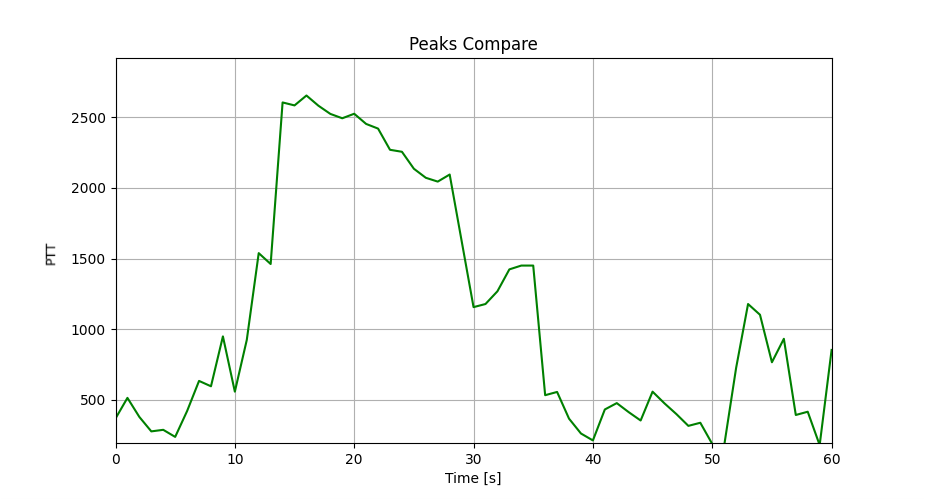
\includegraphics[width=1.0\linewidth]{Peaks_compare.png}
   \caption{Chwilowe różnice czasowe między szczytami EKG i PPG}
    \label{fig:PTT}
\end{figure}

Z wektora wartości wyznacza się statystyki opisowe, obejmujące średnią, określającą przeciętny czas przejścia fali tętna, oraz odchylenie standardowe, wyrażające jego zmienność.

\subsection{Wskaźniki HRV}
Odstępy między kolejnymi uderzeniami serca analizowano niezależnie w obu sygnałach. W elektrokardiografii wykorzystano czas względny, wynikający z okienkowego trybu przetwarzania próbek, natomiast w fotopletyzmografii zastosowano znaczniki systemowe, zapewniając spójność z rejestrowanym przebiegiem oraz umożliwiając synchronizację z innymi źródłami danych. Dla zapisu EKG określono interwały RR, odpowiadające odległościom między załamkami R, a w PPG odstępy międzyuderzeniowe IBI. Na podstawie tych wartości wyznaczono standardowe parametry HRV, przedstawione w formie RR. Analogiczne obliczenia przeprowadzono dla IBI.

\noindent\textit{1) Średnia długość interwału:} 
Średnia arytmetyczna odstępów RR, wyrażona wzorem (4):
\begin{equation}
    Mean = \frac{1}{N} \sum_{i=1}^{N} RR_i
\end{equation}
gdzie $RR_i$ -- $i$-ty odstęp RR, a $N$ – liczba analizowanych odstępów.

\noindent\textit{2) Odchylenie standardowe odstępów NN:} 
Wielkość całkowitej zmienności rytmu serca, obliczana na podstawie wszystkich interwałów RR, wyrażona wzorem (5):
\begin{equation}
    SDNN = \sqrt{\frac{1}{N-1} \sum_{i=1}^{N} (RR_i - Mean)^2}
\end{equation}
gdzie $Mean$ – średnia długość interwału, $RR_i$ – $i$-ty odstęp RR, a $N$ – liczba analizowanych odstępów. 
\newpage
\noindent\textit{3) Pierwiastek kwadratowy z uśrednionych kwadratów różnic kolejnych odstępów NN:} 
Miara stosowana w ocenie krótkoterminowych wahań rytmu serca, wyrażona wzorem (6):
\begin{equation}
    RMSSD = \sqrt{\frac{1}{N-1} \sum_{i=1}^{N-1} (RR_{i+1} - RR_i)^2}
\end{equation}
gdzie $RR_i$ -- $i$-ty odstęp RR, a $N$ – liczba analizowanych odstępów.

\begin{figure}[h]
    \centering
    \begin{subfigure}{0.47\textwidth}
        \centering
        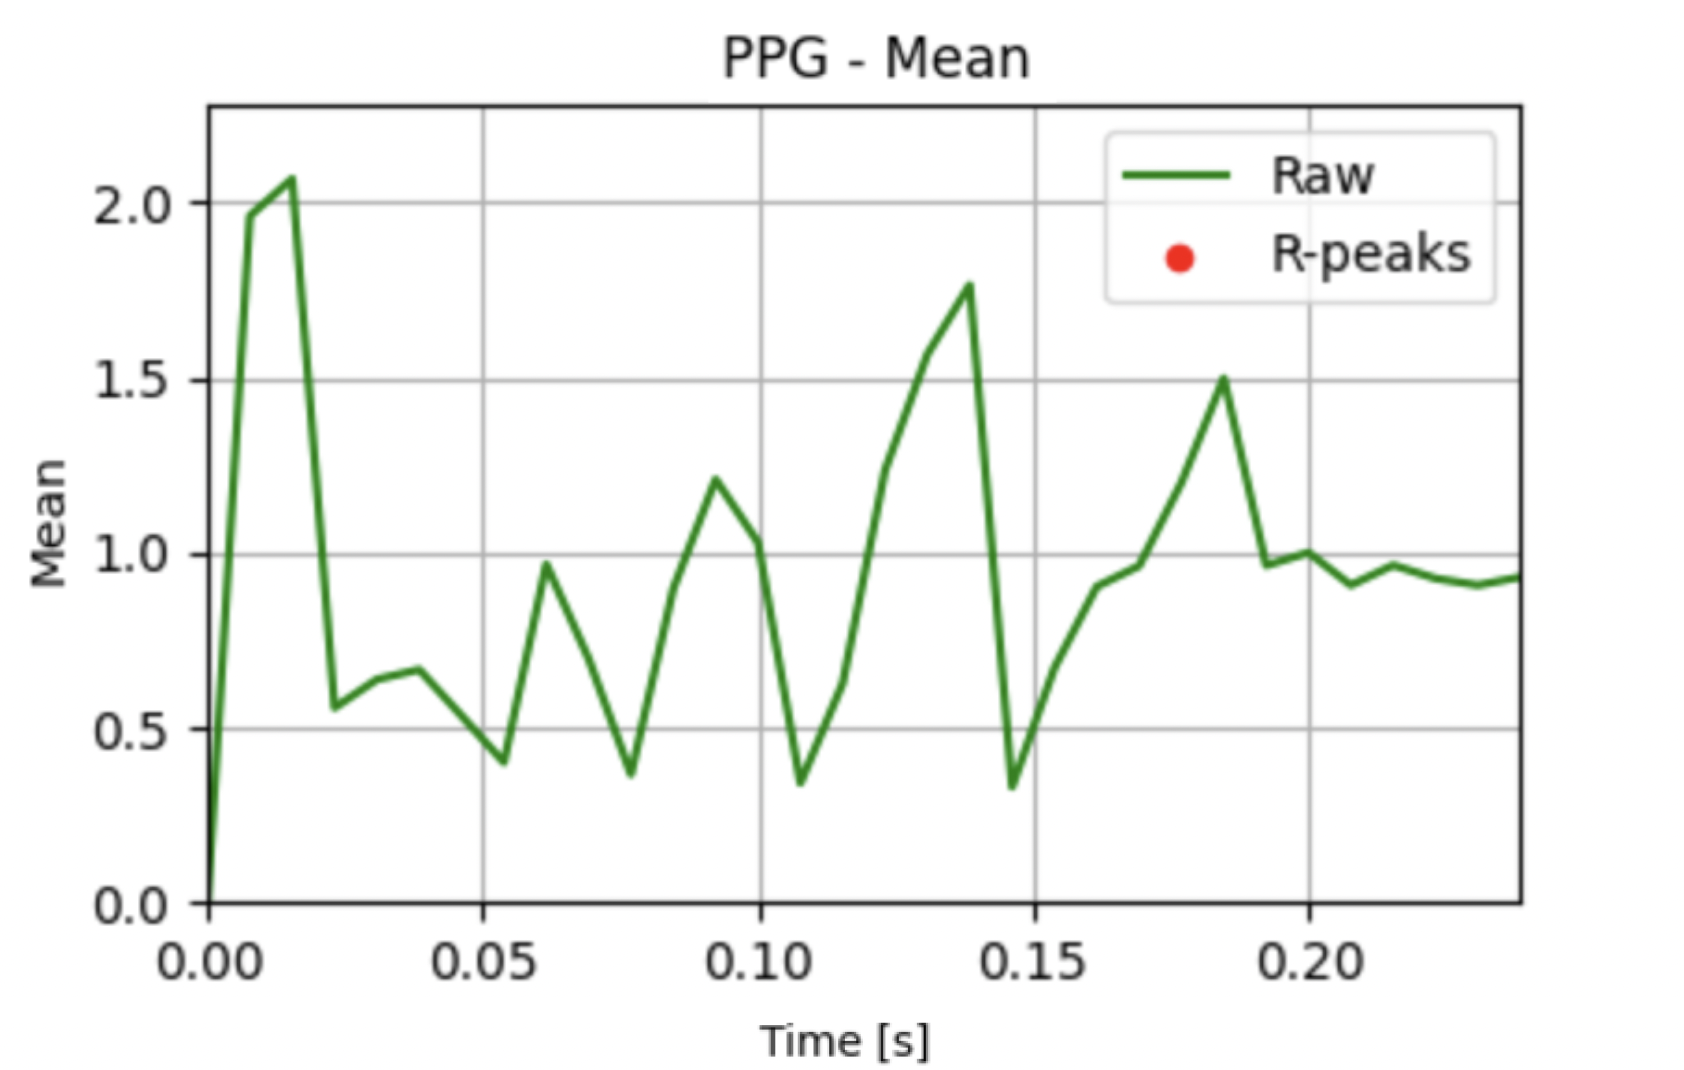
\includegraphics[width=\linewidth]{Mean.png}
        \caption{Średnia długość interwału}
    \end{subfigure}
    
   \vspace{0.2cm} 
    \begin{subfigure}{0.47\textwidth}
        \centering
        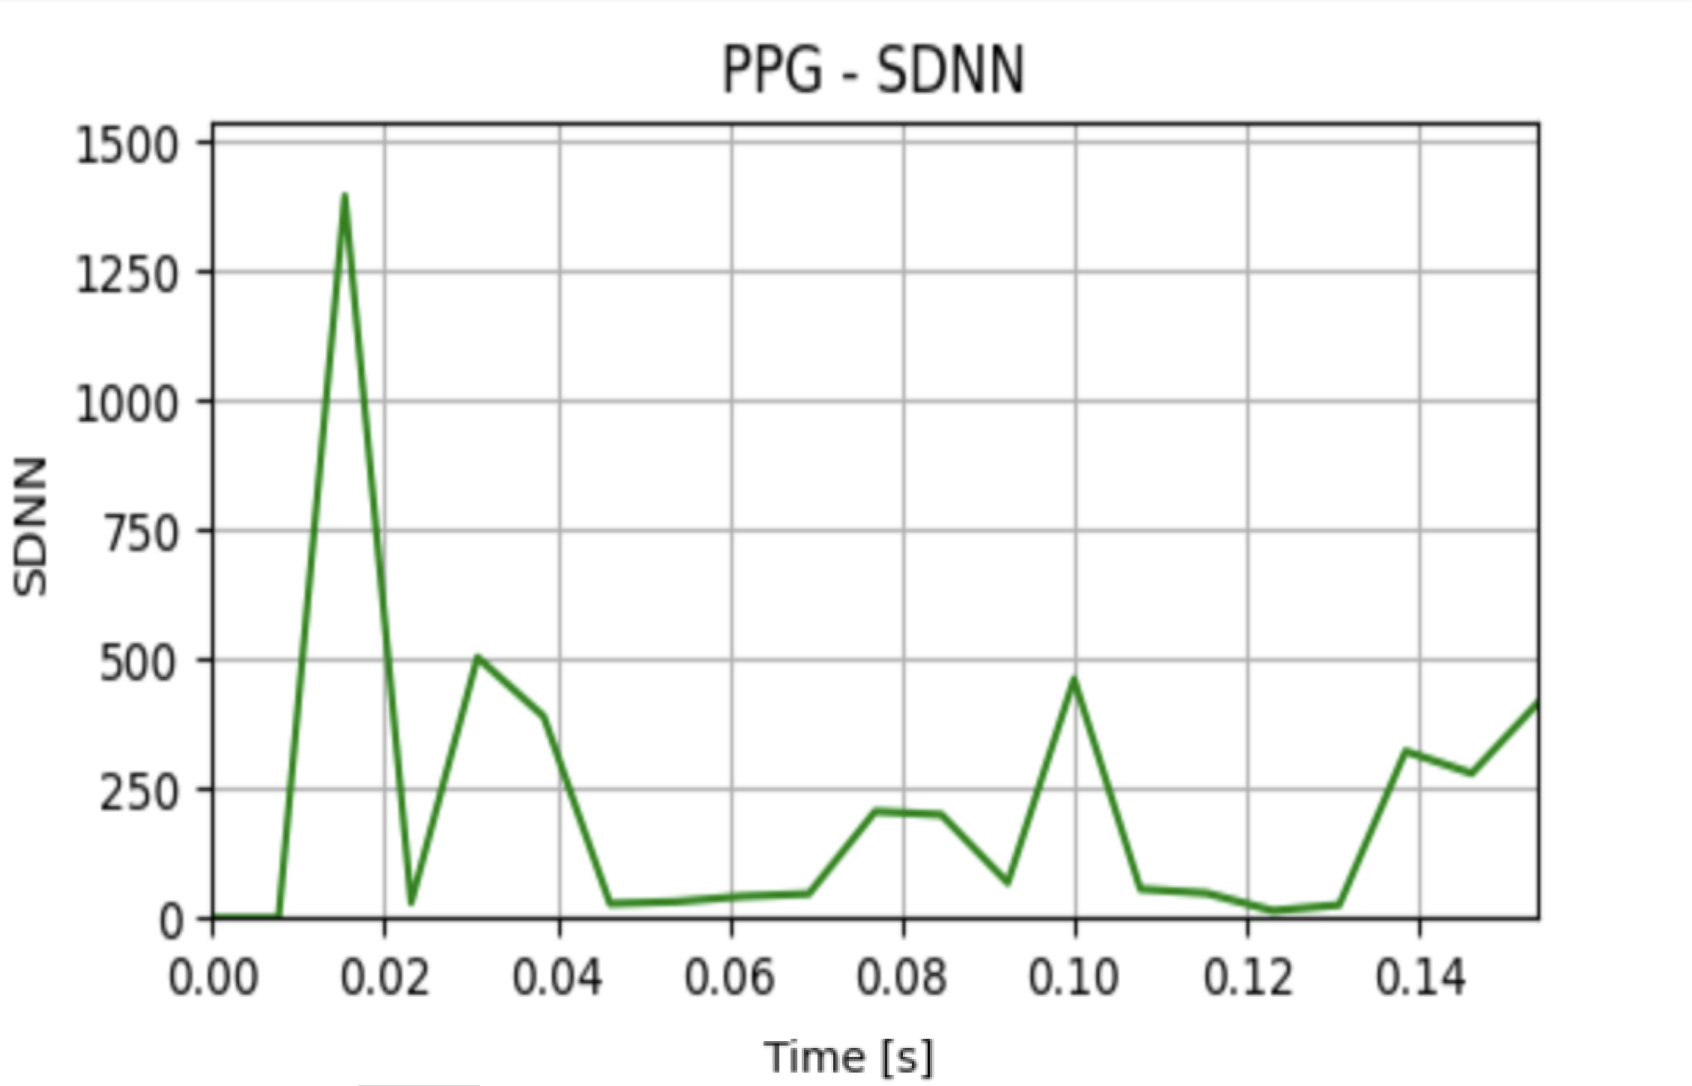
\includegraphics[width=\linewidth]{SDNN.png}
        \caption{Odchylenie standardowe odstępów NN}
    \end{subfigure}
    
    \vspace{0.2cm}  
    \begin{subfigure}{0.47\textwidth}
        \centering
        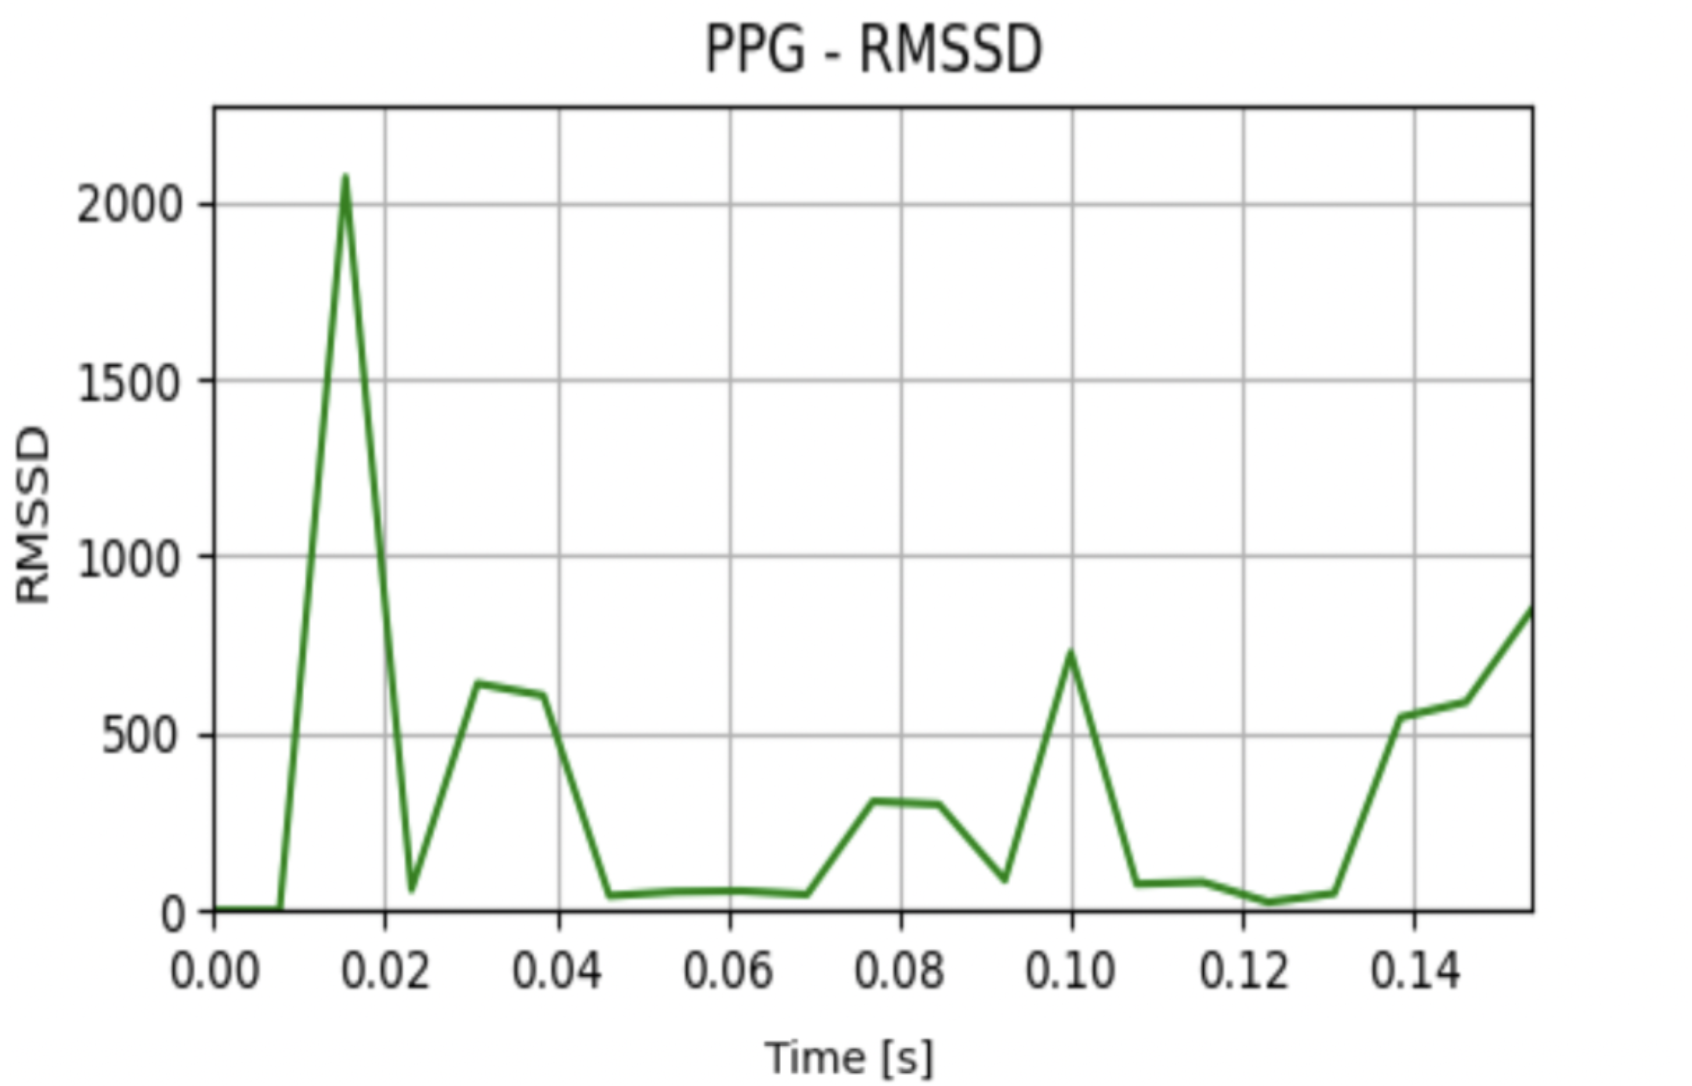
\includegraphics[width=\linewidth]{RMSSD.png}
        \caption{Pierwiastek kwadratowy średniej z kwadratów różnic  odstępów NN}
    \end{subfigure}  
    \caption{Przykładowe przebiegi wskaźników HRV wyznaczone dla PPG}
\end{figure}

\newpage
Do obliczeń w czasie rzeczywistym wykorzystano dynamiczne okno o długości 60 s. Oznaczenia pików oraz odpowiadające im odstępy są aktualizowane w trybie online, natomiast próbki spoza okna są usuwane. Parametry SDNN, RMSSD oraz średnie interwały między uderzeniami serca przedstawiono w postaci wykresów.
%Added na dole:::

Dla porównania przedstawiono również przebiegi wskaźników HRV wyznaczonych z sygnału EKG:

\begin{figure}[h]
    \centering
    \begin{subfigure}{0.47\textwidth}
        \centering
        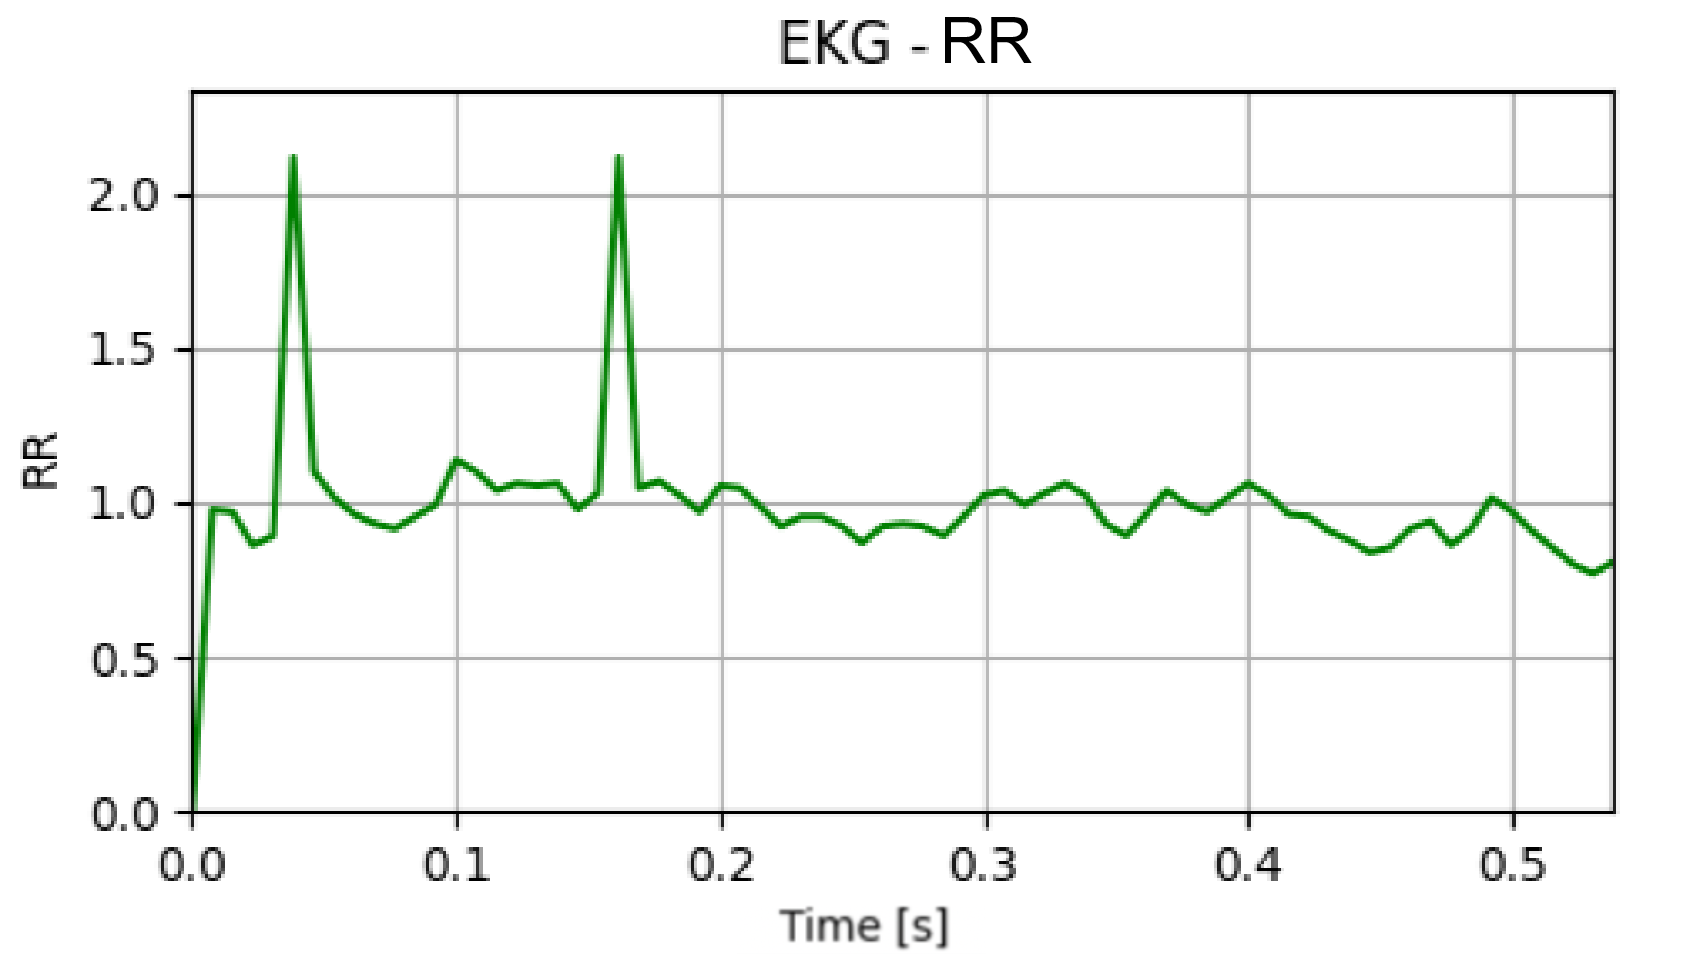
\includegraphics[width=\linewidth]{MEAN_EKG.png}
        \caption{Interwały RR dla EKG}
    \end{subfigure}
    
   \vspace{0.2cm} 
    \begin{subfigure}{0.49\textwidth}
        \centering
        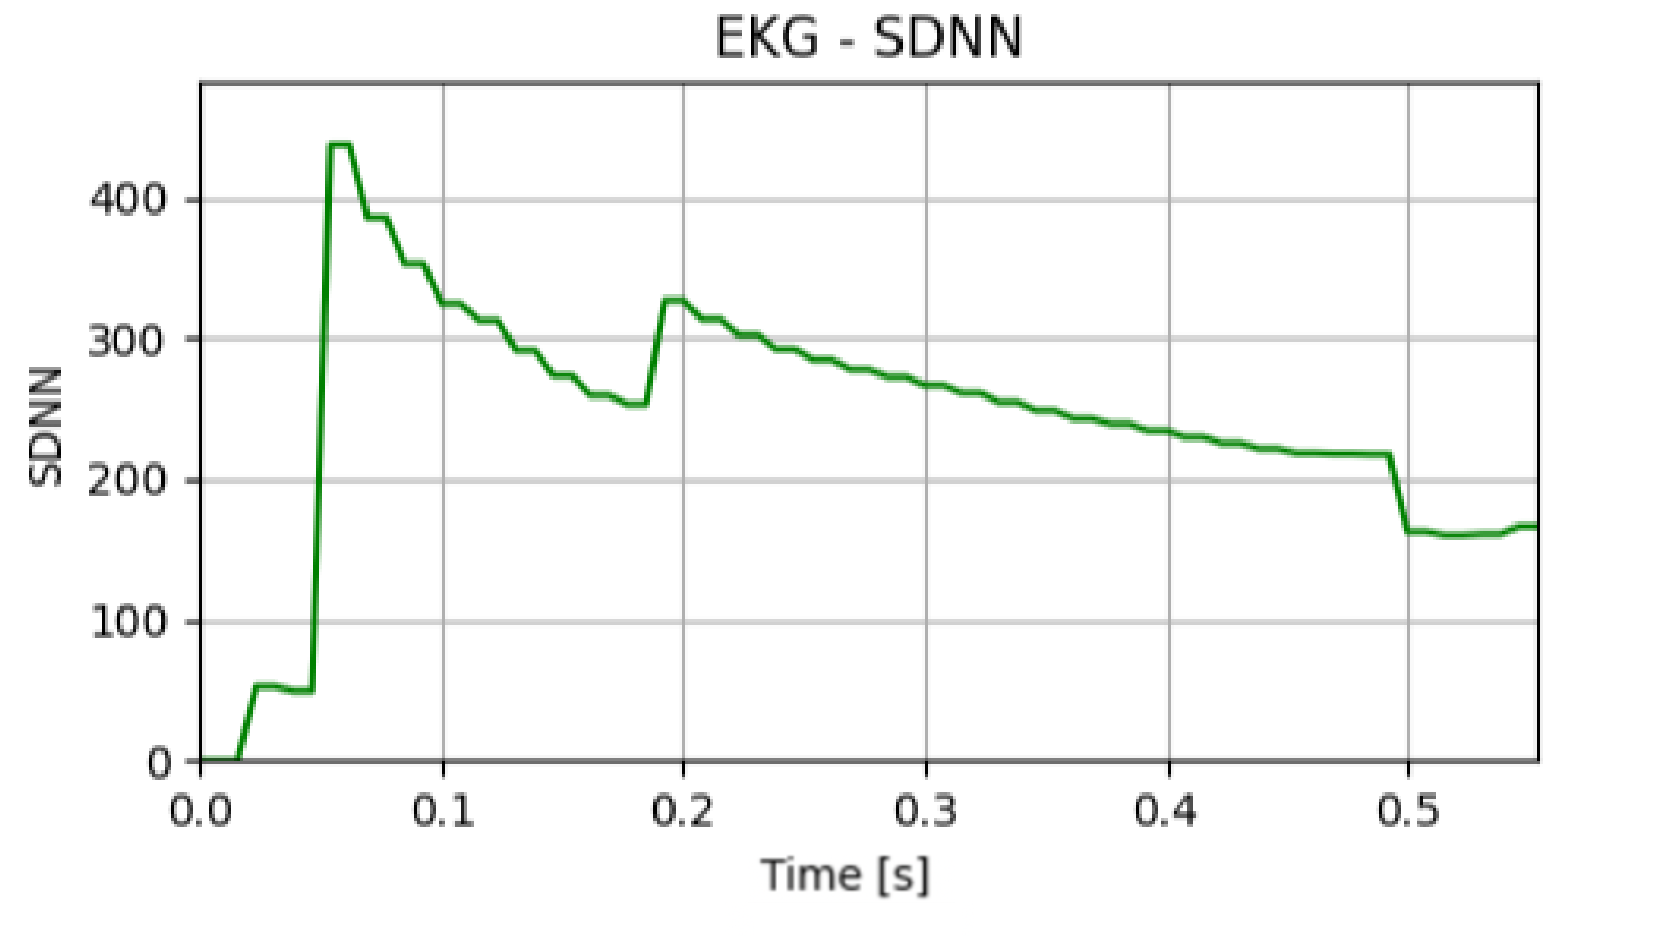
\includegraphics[width=\linewidth]{SDNN_EKG.png}
        \caption{Odchylenie standardowe odstępów NN}
    \end{subfigure}
    
    \vspace{0.2cm}  
    \begin{subfigure}{0.47\textwidth}
        \centering
        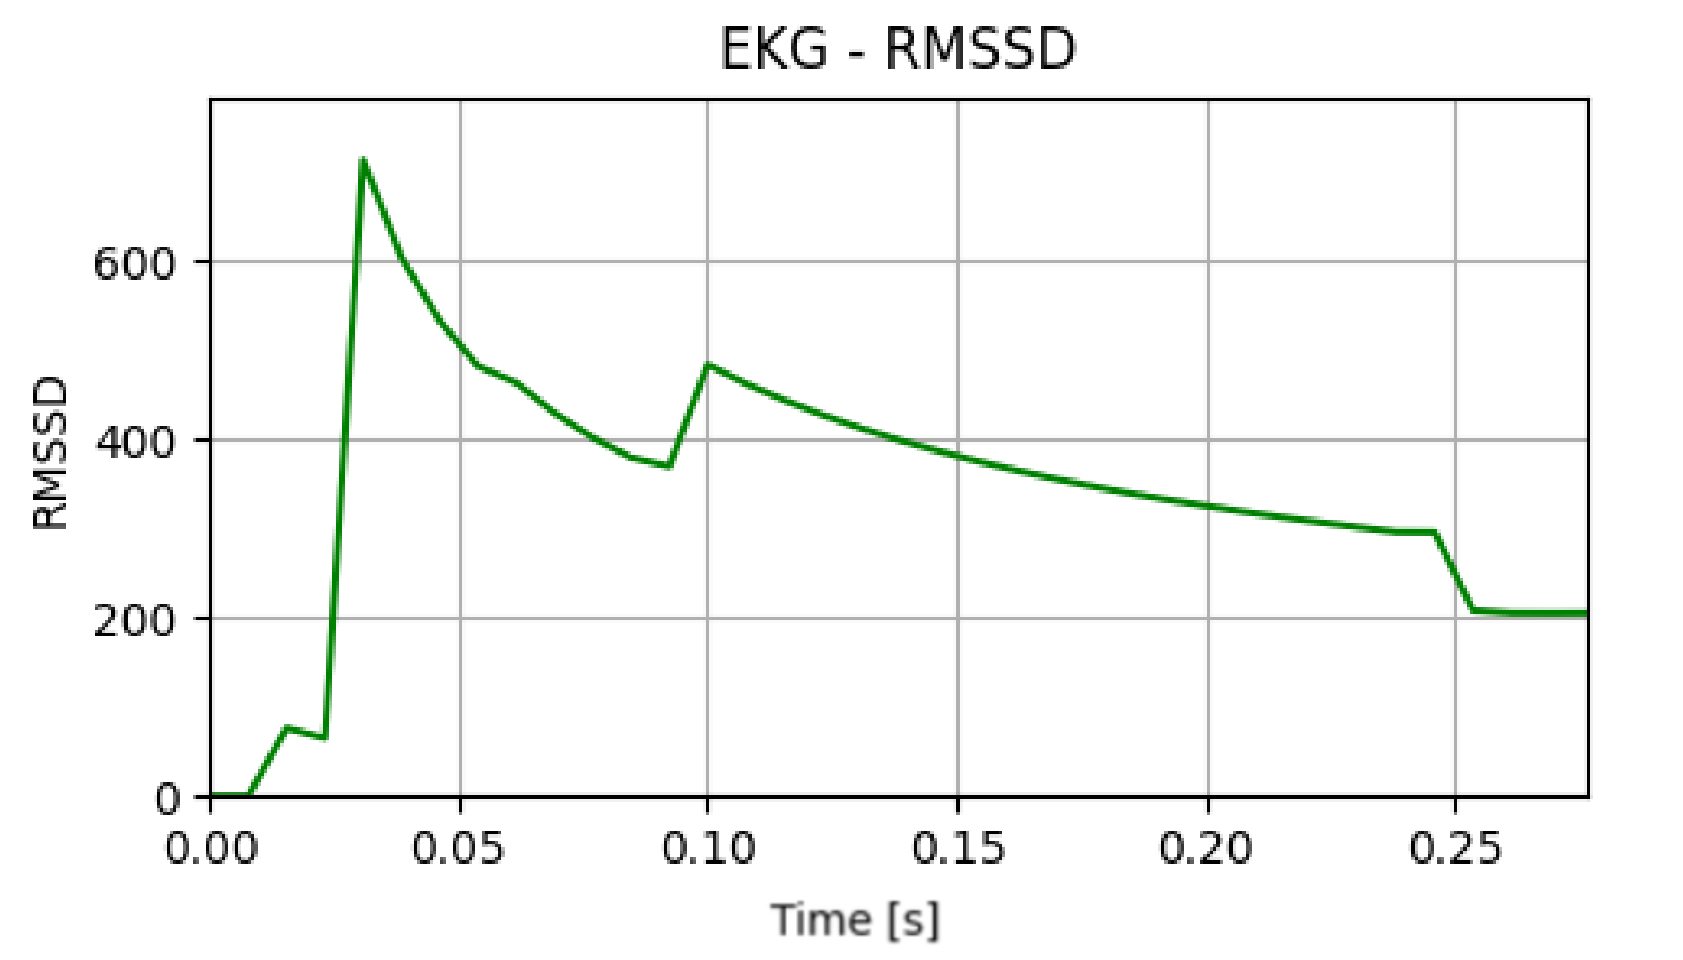
\includegraphics[width=\linewidth]{RMSSD_EKG.png}
        \caption{Pierwiastek kwadratowy średniej z kwadratów różnic  odstępów NN}
    \end{subfigure}  
    \caption{Przykładowe przebiegi wskaźników HRV wyznaczone dla EKG}
\end{figure}

Porównanie wzkaźników HRV dla metody PPG i EKG wykazało, że wartości RMSSD i SDNN wyznaczone z EKG charakteryzują się większą stabilnością i mniejszą podatnością na skoki wartości. W przypadku PPG zauważalne były większe wahania oraz obecność pojedynczych wartości odstających, co wynika z podatności tej metody na zakłócenia, takie jak ruch czy zmienny nacisk palca na kamerę smartfona.

Pomimo większej zmienności w przebiegach PPG, średnie wartości wskaźników (SDNN i RMSSD) były zbliżone do uzyskanych dla EKG. Potwierdza to, że przy odpowiednich warunkach rejestracji PPG może stanowić wiarygodną alternatywę dla EKG w analizie zmienności rytmu serca, choć jego zastosowanie wymaga dodatkowych metod filtracji i kompensacji artefaktów.


\section{Podsumowanie}
Ewaluacja wykazała, że zastosowane architektury splotowe i rekurencyjne zapewniają wysoką zgodność z klasycznymi metodami oraz danymi wzorcowymi, przy jednoczesnym ograniczeniu liczby fałszywych detekcji. %Uzyskane wartości miary F1 potwierdzają skuteczność analizy parametrów sercowo-naczyniowych  w warunkach mobilnych, niezależnie od poziomu aktywności fizycznej.
% fix number2:
%Zaproponowane metody osiągnęły wysoką skuteczność detekcji charakterystycznych punktów sygnału, uzyskując miarę F1 w detekcji załamków R równą 0,9753 dla elektrokardiografii, natomiast dla sygnału fotopletyzmograficznego przy wykrywaniu lokalnych szczytów uzyskano F1 równą 0,9774. %added2
%Średni interwał RR wyznaczony z EKG oraz interwał międzyuderzeniowy IBI z PPG różniły się średnio o około 5 ms. Różnica ta mieści się w granicach błędu pomiarowego i wskazuje na dużą zgodność między sygnałem pozyskiwanym za pomocą czujnika EKG a akwizycją PPG realizowaną smartfonem. %added3
%Wartości podstawowych parametrów HRV (SDNN, RMSSD) obliczone z PPG były bardzo zbliżone do tych z EKG, różnice mieściły się w granicach błędu pomiarowego.
Zaproponowane modele osiągnęły wysoką precyzję w detekcji kluczowych punktów sygnału, uzyskując miarę F1 na poziomie 0,9753 dla załamków R w sygnale EKG oraz 0,9774 dla szczytów fali w przebiegu PPG.
Wysoka dokładność detekcji pików w sygnale fotopletyzmograficznym świadczy o dużym potencjale tej metody do wiarygodnego szacowania interwałów międzyuderzeniowych IBI, które są odpowiednikiem interwałów RR z EKG.

Systemy rejestracji sygnałów biomedycznych, wspierane metodami uczenia maszynowego, wykazują potencjał w monitorowaniu stanu zdrowia w czasie rzeczywistym. Kolejne etapy prac powinny koncentrować się na zwiększenie odporności algorytmów detekcji na zakłócenia środowiskowe, w tym artefakty ruchowe, szumy oraz zmienne warunki fizjologiczne. Równocześnie kluczowe jest opracowanie mechanizmów integracji z zaawansowanymi systemami telemedycznymi, umożliwiającymi przesyłanie oraz analizę danych w sposób ciągły. Zastosowanie tych rozwiązań może wspierać wczesną identyfikację zaburzeń rytmu serca oraz wspomagać proces podejmowania decyzji klinicznych.

Warto jednak podkreślić, że choć modele trenowano na danych uwzględniających zakłócenia, takie jak nagłe ruchy ciała czy drobne poruszenia palca, ich walidacja odbyła się w warunkach kontrolowanych. Kluczowym ograniczeniem jest zatem niepewność co do zachowania systemu w warunkach rzeczywistych, zwłaszcza podczas intensywnej aktywności fizycznej, gdzie ruch staje się dominującym źródłem zniekształceń. Problem ten jest szczególnie widoczny w sygnale PPG, gdzie niestabilny kontakt czujnika ze skórą może prowadzić do znacznych błędów pomiarowych. Możliwe usprawnienia, które pozwolą zniwelować wpływ zakłóceń na rezultaty badań to: zastosowanie filtrów adaptacyjnych, które dynamicznie dostosowują swoje działanie do charakterystyki szumu w sygnale, lub wykorzystanie bardziej złożonych modeli uczenia głębokiego do przetwarzania zróżnicowanych danych.

\newpage

Opracowany system wraz z kodem źródłowym został udostępniony publicznie w repozytoriach na GitHub pod adresami:

\noindent
\href{https://github.com/JanBancerewicz/PPGbetter}{https://github.com/JanBancerewicz/PPGbetter}
\href{https://github.com/JanBancerewicz/research-project}{https://github.com/JanBancerewicz/research-project}.

 

\begin{thebibliography}{1}
\bibitem{1}
C. Bronzino, J. D. Bronzino, “The Biomedical Engineering Handbook: Biomedical Signal Analysis”
\bibitem{2}
R. R. Sharma, R. B. Pachori, “Baseline Wander and Power Line Interference Removal from ECG Signals”, 2018
\bibitem{3}
S. Sörnmo, L. Laguna, “Bioelectrical Signal Processing in Cardiac and Neurological Applications”, 2005
\bibitem{4}
P. Podder, M. M. Hasan, M. R. Islam, M. Sayeed, “Design and Implementation of Butterworth, Chebyshev-I and Elliptic Filter for Speech Signal Analysis”, 2020
\bibitem{5}
M. R. Keshtkaran, Z. Yang, “A fast, robust algorithm for power line interference cancellation in neural recording”, 2014
\bibitem{6}
S. K. Mitra, “Digital Signal Processing: A Computer-Based Approach”
\bibitem{7}
Y. Yue, “An effective electrocardiogram segments denoising method based on EEMD, EMD, and wavelet packet”, IET Signal Processing
\bibitem{8}
S. Haykin, “Adaptive Filter Theory”, 5th ed., Pearson, 2013
\bibitem{9}
A. Hyvärinen, E. Oja, “Independent component analysis: algorithms and applications”
\bibitem{10}
O. Faust, U. R. Acharya, H. Adeli, A. Adeli, “Deep learning for healthcare applications based on physiological signals: A review”
\bibitem{11}
A. Boulif et al., “A literature review: ECG-based models for arrhythmia detection using AI techniques”, 2023
\bibitem{12}
Z. Ebrahimi, “A review on deep learning methods for ECG arrhythmia detection”
\bibitem{13}
D. A. Coast, R. M. Stern, G. G. Cano, S. A. Briller, “An approach to cardiac arrhythmia analysis using hidden Markov models”
\bibitem{14}
K. Kazemi, “Robust PPG Peak Detection Using Dilated Convolutional Neural Networks”
\bibitem{15}
S. Ikram et al., “Transformer-based ECG classification for early detection of cardiac arrhythmias”
\bibitem{16}
C. V. Nguyen, C. D. Do, “Transfer learning in ECG diagnosis: Is it effective?”
\bibitem{17}
W. Wang, L. Najafizadeh, “Ultra-Short Term Heart Rate Variability Estimation Using PPG and End-to-End Deep Learning”, 2024
\bibitem{18}
J. Xu, Y. Zhang, W. Wang, M. Xie, D. Zhu, “A Comprehensive PPG-based Dataset for HR/HRV Studies”, 2025
\bibitem{19}
B. De Ridder et al., “Smartphone Apps Using Photoplethysmography for Heart Rate Measurement: Systematic Review”
\bibitem{20}
J. D. Mather et al., “Validity of Resting Heart Rate Derived from Contact-Based Smartphone PPG”, 2024
\bibitem{21} 
Polar Electro, “Polar H10 heart rate sensor,” 2025
\bibitem{22} 
W. M. Laghari, M. Baloch, M. Mengal, S. Shah, “Performance Analysis of Analog Butterworth Low Pass Filter as Compared to Chebyshev Type-I Filter, Chebyshev Type-II Filter and Elliptical Filter”
\bibitem{23} 
S. Chakraborty, K. K. Jha, A. Patra, “Design of IIR Digital Highpass Butterworth Filter using Analog to Digital Mapping Technique”
\bibitem{24} 
G. Lenis, N. Pilia, A. Loewe, W. H. W. Schulze, O. Dössel, “Comparison of Baseline Wander Removal Techniques considering the Preservation of ST Changes in the Ischemic ECG: A Simulation Study”
\bibitem{25} 
R. J. Martis, U. R. Acharya, H. Adeli, “Current methods in electrocardiogram characterization”
\bibitem{26} 
M. A. F. Pimentel et al., “Toward a robust estimation of heart rate from wrist-type PPG signals”, 2016
\bibitem{27} 
J. Pan and W. J. Tompkins, “A real-time QRS detection algorithm”
\end{thebibliography}
\end{document}


